\documentclass[pdflatex,sn-mathphys]{sn-jnl}
\usepackage[utf8]{inputenc}
\usepackage{tipa}
\usepackage{lineno}

\jyear{2025}

\raggedbottom

\newcommand{\myvec}[1]{\ensuremath{\begin{pmatrix}#1\end{pmatrix}}}
\usepackage{amsmath}
\DeclareMathOperator{\sign}{sign}

\begin{document}

\title[Personalising language embeddings]{Personalising language embeddings reveals structured individual differences in how humans represent meaning}
%\title[Modelling individual semantic spaces]{Individual differences in human semantics are reliable, structured and learnable}

\author*[1,2]{\fnm{Fabian} \sur{Schneider}}\email{fabian@fschneider.dev}
\author[1,2,3]{\fnm{Helen} \sur{Blank}}\email{helen.blank@rub.de}

\affil[1]{\orgdiv{Institute for Systems Neuroscience}, \orgname{University Medical Centre Hamburg-Eppendorf}}%, \orgaddress{\street{Martinistr. 52}, \city{Hamburg}, \postcode{20246}, \state{Hamburg}, \country{Germany}}}
\affil[2]{\orgdiv{Faculty of Psychology}, \orgname{Ruhr University Bochum}}%, \orgaddress{\street{Universitätsstr. 150}, \city{Bochum}, \postcode{44801}, \state{North-Rhine Westphalia}, \country{Germany}}}
\affil[3]{\orgdiv{Research Center One Health Ruhr}, \orgname{University Alliance Ruhr}}%, \orgaddress{\street{Universitätsstr. 150}, \city{Bochum}, \postcode{44801}, \state{North-Rhine Westphalia}, \country{Germany}}}

\abstract{People differ in the meanings they associate with words, but how these differences are organised across concepts remains unclear. Here we tested whether individual semantic judgements reveal stable, generalisable structure and whether personalising language embeddings can capture it. We measured semantic geometries using multiple-arrangement judgements across multiple sessions. Participants’ judgements were more similar within and across sessions than to those of other people or embeddings. Adapting embeddings to individuals using ten minutes of behavioural data improved prediction of held-out judgements by approximately 40\%, with benefits extending to word pairs and words absent from training. Demographic and experiential characteristics predicted both embedding-human divergence and individual departures from shared semantic structure. Individual departures varied systematically across semantic domains and word properties. These findings show that individual semantic differences contain stable, learnable structure that extends across concepts and is associated with demographic, experiential and word characteristics.}

\keywords{semantics; individual differences; representations; embeddings; artificial intelligence}

\maketitle

\linenumbers

\section{Introduction}\label{introduction}
Humans communicate through a shared vocabulary, but the experiences engendering words with meaning may vary between individuals\cite{Johns2024,Marti2023,Guitard2027,Schwartz2013,Jansen2026}: One person may associate \textit{coffee} primarily with \textit{work} and \textit{alertness}, whereas another may associate it with \textit{conversation} and \textit{friendship}. Such variation in meaning is expected under theories of semantic cognition in which semantic representations are shaped by regularities in linguistic, perceptual and social experience\cite{Binder2011,Meteyard2012,Reilly2025}. Indeed, learning and memory are known to be sensitive to the statistical structure of what people encounter\cite{Summerfield2025,Cain2025} and interindividual differences in semantic perception have been reported\cite{Johns2024,Marti2023}. Yet, the organisation of individual semantic differences remains unclear: Do a person's semantic judgements reveal systematic tendencies that extend across concepts, and are these tendencies shared across people with similar backgrounds and experiences? Addressing these questions requires distinguishing the semantic organisation shared across humans from systematic departures specific to an individual.

Representing meaning as geometry provides a way to investigate the organisation of semantic spaces\cite{glove,Gentzkow2019}. Distributional word and language embeddings provide compact vector-space descriptions of lexical and conceptual relations\cite{glove}. They capture substantial shared structure in human semantic representations\cite{Goldstein2024,Kumar2024,Mischler2024} and have become a standard operationalisation of meaning in the social\cite{Xu2026,Kozlowski2019,Caliskan2017,Freden2024,Garg2017,Rheault2020}, behavioural\cite{Grand2022,Olson2021,Wulff2025,Lee2025}, neural\cite{Huth2016,Heilbronetal2022,King2025,Tang2023,Tang2025} and computer sciences\cite{Karpukhin2020,Radford2021,Reimers2019}. Yet, they are trained on large corpora whose distributional statistics, genres and social histories shape the meaning they encode\cite{Bender2021,Atari2023,Paullada2021}. Even an otherwise unbiased embedding pools text produced by millions of individuals with heterogeneous constraints in the form of their lived experiences\cite{Atari2023,Bosch2026}. Agreement with human judgements at the group level therefore leaves open how adequately an embedding describes any particular person. Personalising embeddings offers a potential way to close this gap. Whether such adaptation can recover individual semantic organisation depends on its ability to predict judgements beyond those used for training. Comparing these predictions with predictions from embeddings adapted to other people can establish whether the generalisable structure is specific to the individual. Therefore, this approach could both reveal how semantic differences are organised and extend the ability of embeddings to model individual meaning.

Here, we investigate individual semantic organisation using multiple-arrangement judgements, in which participants repeatedly arranged words according to their perceived semantic similarity. In an initial cohort tested in two sessions ($N = 30$), participants exhibited stable individual differences beyond the structure captured by widely used embeddings or other participants' judgements. We developed a lightweight adaptation model that learns participant-specific transformations of an existing embedding while regularising departures from its original structure. With as little as ten minutes of behavioural training data, personalisation improved predictions of semantic judgements, including those involving words for which no judgements had been used in training. In an independent sample ($N = 303$), demographic and experiential characteristics predicted both embedding-human alignment and interindividual differences between participants. Non-linear transformations predicted held-out judgements better than parameter-matched linear transformations, indicating that individual differences reflect conceptually local variation. The benefits of non-linear personalisation varied across semantic domains and word properties, and participants' experiential characteristics predicted their distribution across domains. 

Together, these findings show that individual semantic differences contain stable structure that extends across concepts and is associated with demographic and experiential characteristics. Personalised embeddings capture this structure from sparse behavioural observations and predict previously unmeasured judgements, extending their role as models of shared semantic organisation to account for systematic variation in individual meaning.

\section{Results}\label{results}

\begin{figure}[H]%
\centering
\hspace*{0.2cm}
\noindent\makebox[\textwidth]{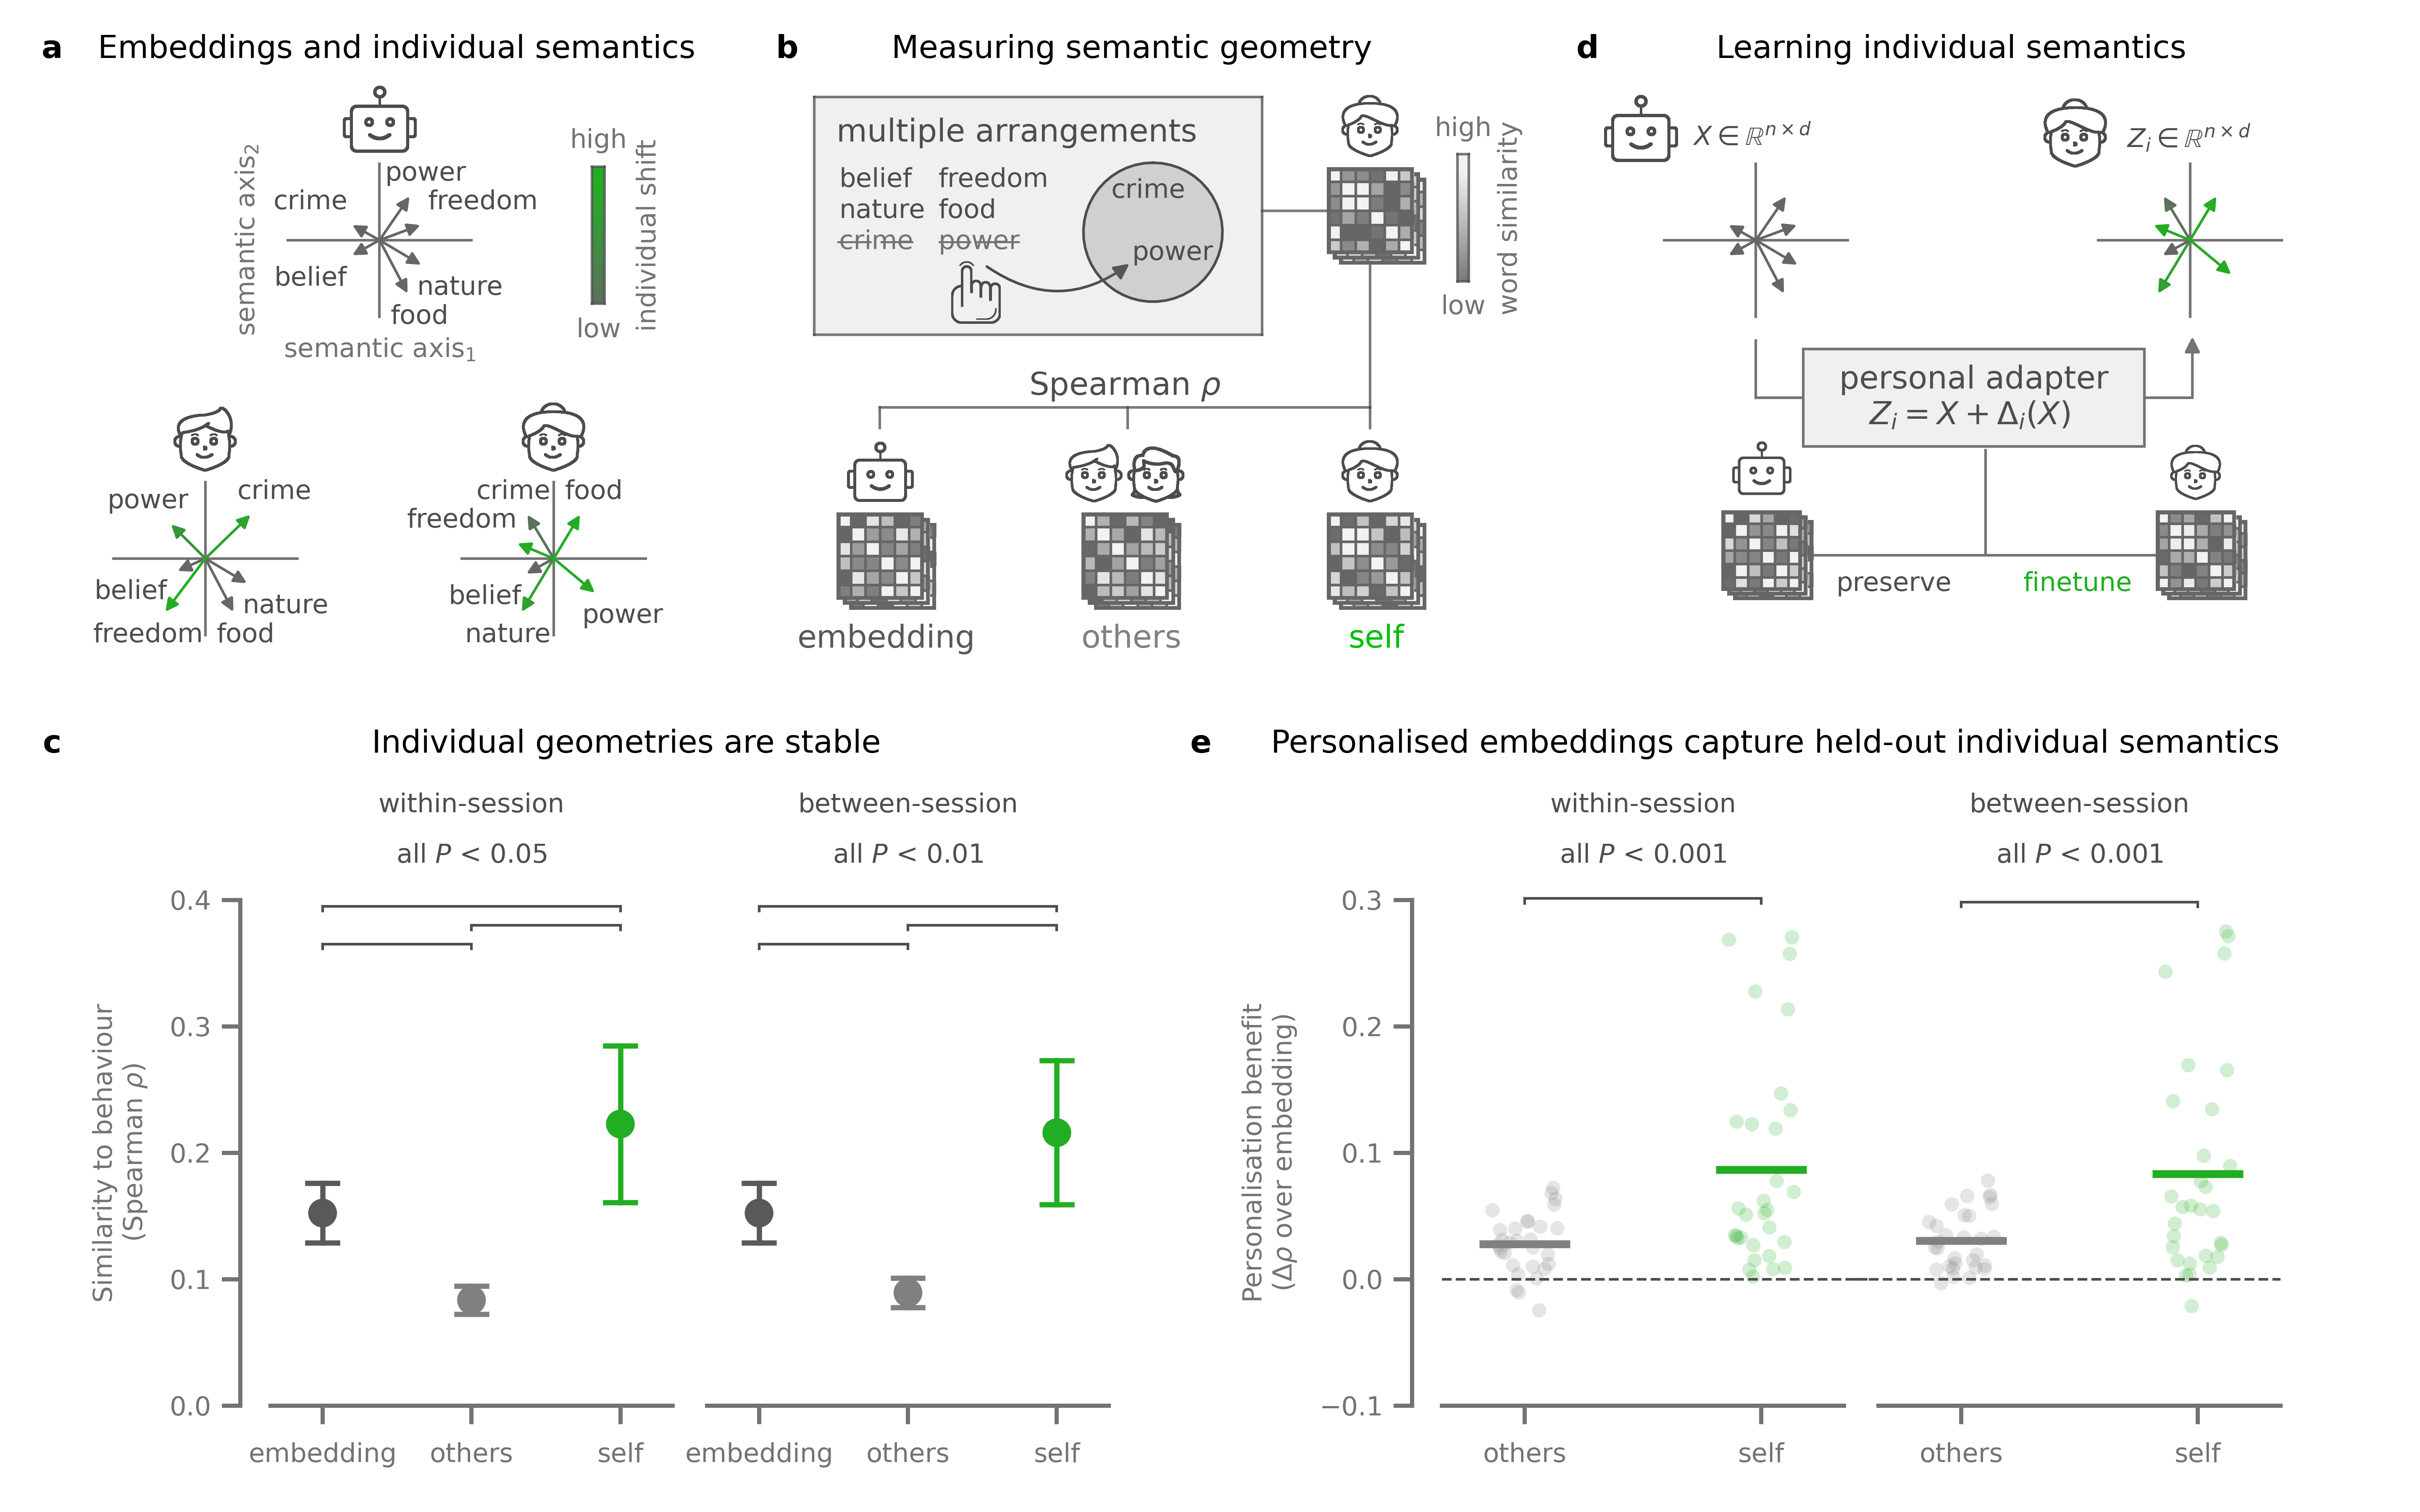
\includegraphics[width=0.9\paperwidth]{fig1.png}}
\caption{
\textbf{Individual semantic geometries are stable and can be recovered through personalisation.}
\textbf{a,} Word and language embeddings are commonly used as geometric representations of lexical and conceptual meaning. However, a single embedding space collapses across heterogeneous language histories, cultural backgrounds, and individual experiences, and may therefore diverge from the semantic geometry of individual people.
\textbf{b,} Participants completed a multiple-arrangement task in which they arranged words by perceived semantic similarity. The task was completed twice in separate sessions. From these arrangements, we computed split-half representational similarity matrices and compared each participant's semantic geometry with three reference geometries: an off-the-shelf embedding, the geometries of other participants and the participant's own held-out judgements. All similarities were computed as Spearman rank correlations, such that higher values indicate greater agreement in the relative ordering of word-pair similarities.
\textbf{c,} Participants were more similar to their own held-out judgements than to either the embedding model or other participants, both within sessions and across sessions. Dots show means; error bars indicate 95\% confidence intervals.
\textbf{d,} Overview of the individual personalisation approach. Lightweight adapters were trained to transform an initial embedding space into a personalised embedding space for each participant. Training balanced preservation of the original embedding geometry with matching the participant's behavioural geometry.
\textbf{e,} Personalisation benefit was quantified as the improvement in embedding-participant similarity relative to the original embedding geometry (\(\Delta\)Spearman \(\rho\)). Participant-specific adapters produced larger benefits than cross-participant adapters, both within the same session and across sessions.
}\label{fig1}
\end{figure}

\subsection{Semantic judgements reveal stable individual structure}
We first asked whether multiple-arrangement judgements recover reliable individual semantic geometries and how closely these geometries are captured by semantic embeddings (Fig.~\ref{fig1}a,b). Participants ($N = 30$; see \nameref{participants}) completed two multiple-arrangement sessions in which they repeatedly arranged words according to their perceived semantic similarity. The two sessions were completed on separate occasions ($M = 22.07\pm2.73$ hours; see \nameref{procedure}). The word set was selected to span smooth semantic transitions between key semantic domains such as \textit{nature}, \textit{technology}, \textit{relationships}, \textit{religion}, \textit{cuisine}, \textit{politics} and \textit{fashion} (see \nameref{materials}).

Distances between words on a board described each participant's semantic geometry. For words shared across boards, we used Spearman's $\rho$ to compare these distances with three references (Fig.~\ref{fig1}b, \nameref{geometries}): distances in an off-the-shelf embedding (\textit{embedding-participant similarity}; \texttt{GloVe}\cite{glove} as primary embedding), distances in other participants' arrangements (\textit{others-participant similarity}), and distances on a different board completed by the same participant (\textit{self-similarity}). 

Off-the-shelf embeddings captured reliable aspects of individual semantic geometry: embedding-participant correlations were consistently above zero ($\rho = 0.152\pm0.009$, $P < 0.001$, sign-flip permutation test). However, participants' own held-out judgements provided a substantially better account of their semantic geometry than the embedding model. Within-session self-similarity exceeded embedding-participant similarity by 46\% ($\Delta\rho = 0.070\pm0.028, P < 0.01$, sign-flip permutation test; Fig.~\ref{fig1}c). Self-similarity also exceeded others-participant similarity by 167\% ($\Delta\rho = 0.139\pm0.031, P < 0.001$, sign-flip permutation test; Fig.~\ref{fig1}c), indicating that the additional explainable structure was not merely shared across participants but reflected reliable individual variation instead.

We next tested whether these individual geometries were stable across time. Repeating the analysis across the two sessions yielded the same pattern: participants were more similar to their own judgements from the other session than to either the embedding or the group (all $P < 0.01$, sign-flip permutation tests; Fig.~\ref{fig1}c). Thus, multiple arrangement judgements revealed stable individual semantic geometries that were only partially captured by off-the-shelf embeddings.

Finally, we asked whether this pattern depended on the use of a static embedding model. We therefore repeated the analyses using embeddings derived from \texttt{T5}\cite{t5-large} and \texttt{E5}\cite{e5-large} (see \nameref{embeddings}). The results were qualitatively unchanged: across participants, self-similarity exceeded embedding-participant similarity and others-participant similarity (all $P < 0.05$, sign-flip permutation tests; Supplementary Fig.~1). These findings indicate that the divergence between human and off-the-shelf embeddings cannot be attributed solely to embedding-specific confounds.

\subsection{Personalised embeddings capture stable individual semantic structure}
We next asked whether a person's semantic judgements reveal systematic tendencies that generalise across concepts. If so, a continuous transformation should capture the shift from shared to individual semantic space. Therefore, we tested whether off-the-shelf embeddings could be adapted to individual participants using sparse behavioural data. We trained an adapter to adjust word positions in the original embedding so that distances between words better matched that participant's judgements, while penalising departures from the original geometry (Fig.~\ref{fig1}d). Because the adapter learns a transformation that can be applied to any word vector, we could evaluate its predictions on held-out boards and compare them with predictions from the original embedding and from other participants' adapters (see \nameref{implementation}).

For held-out boards, embedding-participant correlations were consistently above zero ($\rho = 0.155\pm0.006$, $P < 0.001$, sign-flip permutation test). Yet, personalised embeddings captured semantic geometries of held-out boards markedly better than off-the-shelf embeddings or those trained on other participants. Within-session self-similarity exceeded embedding-participant similarity by 56\% ($\Delta\rho = 0.087\pm0.015$) and others-participant similarity by 32\% ($\Delta\rho = 0.059\pm0.014$, all $P < 0.001$, sign-flip permutation tests; Fig.~\ref{fig1}e). This indicated that individual adapters could indeed learn structured variation in individual semantic spaces and that adapters could generalise beyond trained relations. 

To test the stability of individual adapters, we repeated these analyses when training adapters on one session and testing them on the other. Results showed the same pattern of benefits (all $P < 0.001$, sign-flip permutation tests; Fig.~\ref{fig1}e), confirming that learned individual adapters were stable across time.

Next, we confirmed that personalisation yielded similar benefits in modern, transformer-derived embeddings. This is non-trivial given that modern embeddings tend to have greatly increased dimensionality, making the adaptation function particularly challenging to learn. Yet, here we also observed the same pattern: embedding-participant correlations were consistently above zero, while self-similarity exceeded embedding-participant similarity and others-participant similarity (all $P < 0.001$, sign-flip permutation tests; Supplementary Fig.~2). 

\begin{figure}[H]%
\centering
\hspace*{0.0cm}
\noindent\makebox[\textwidth]{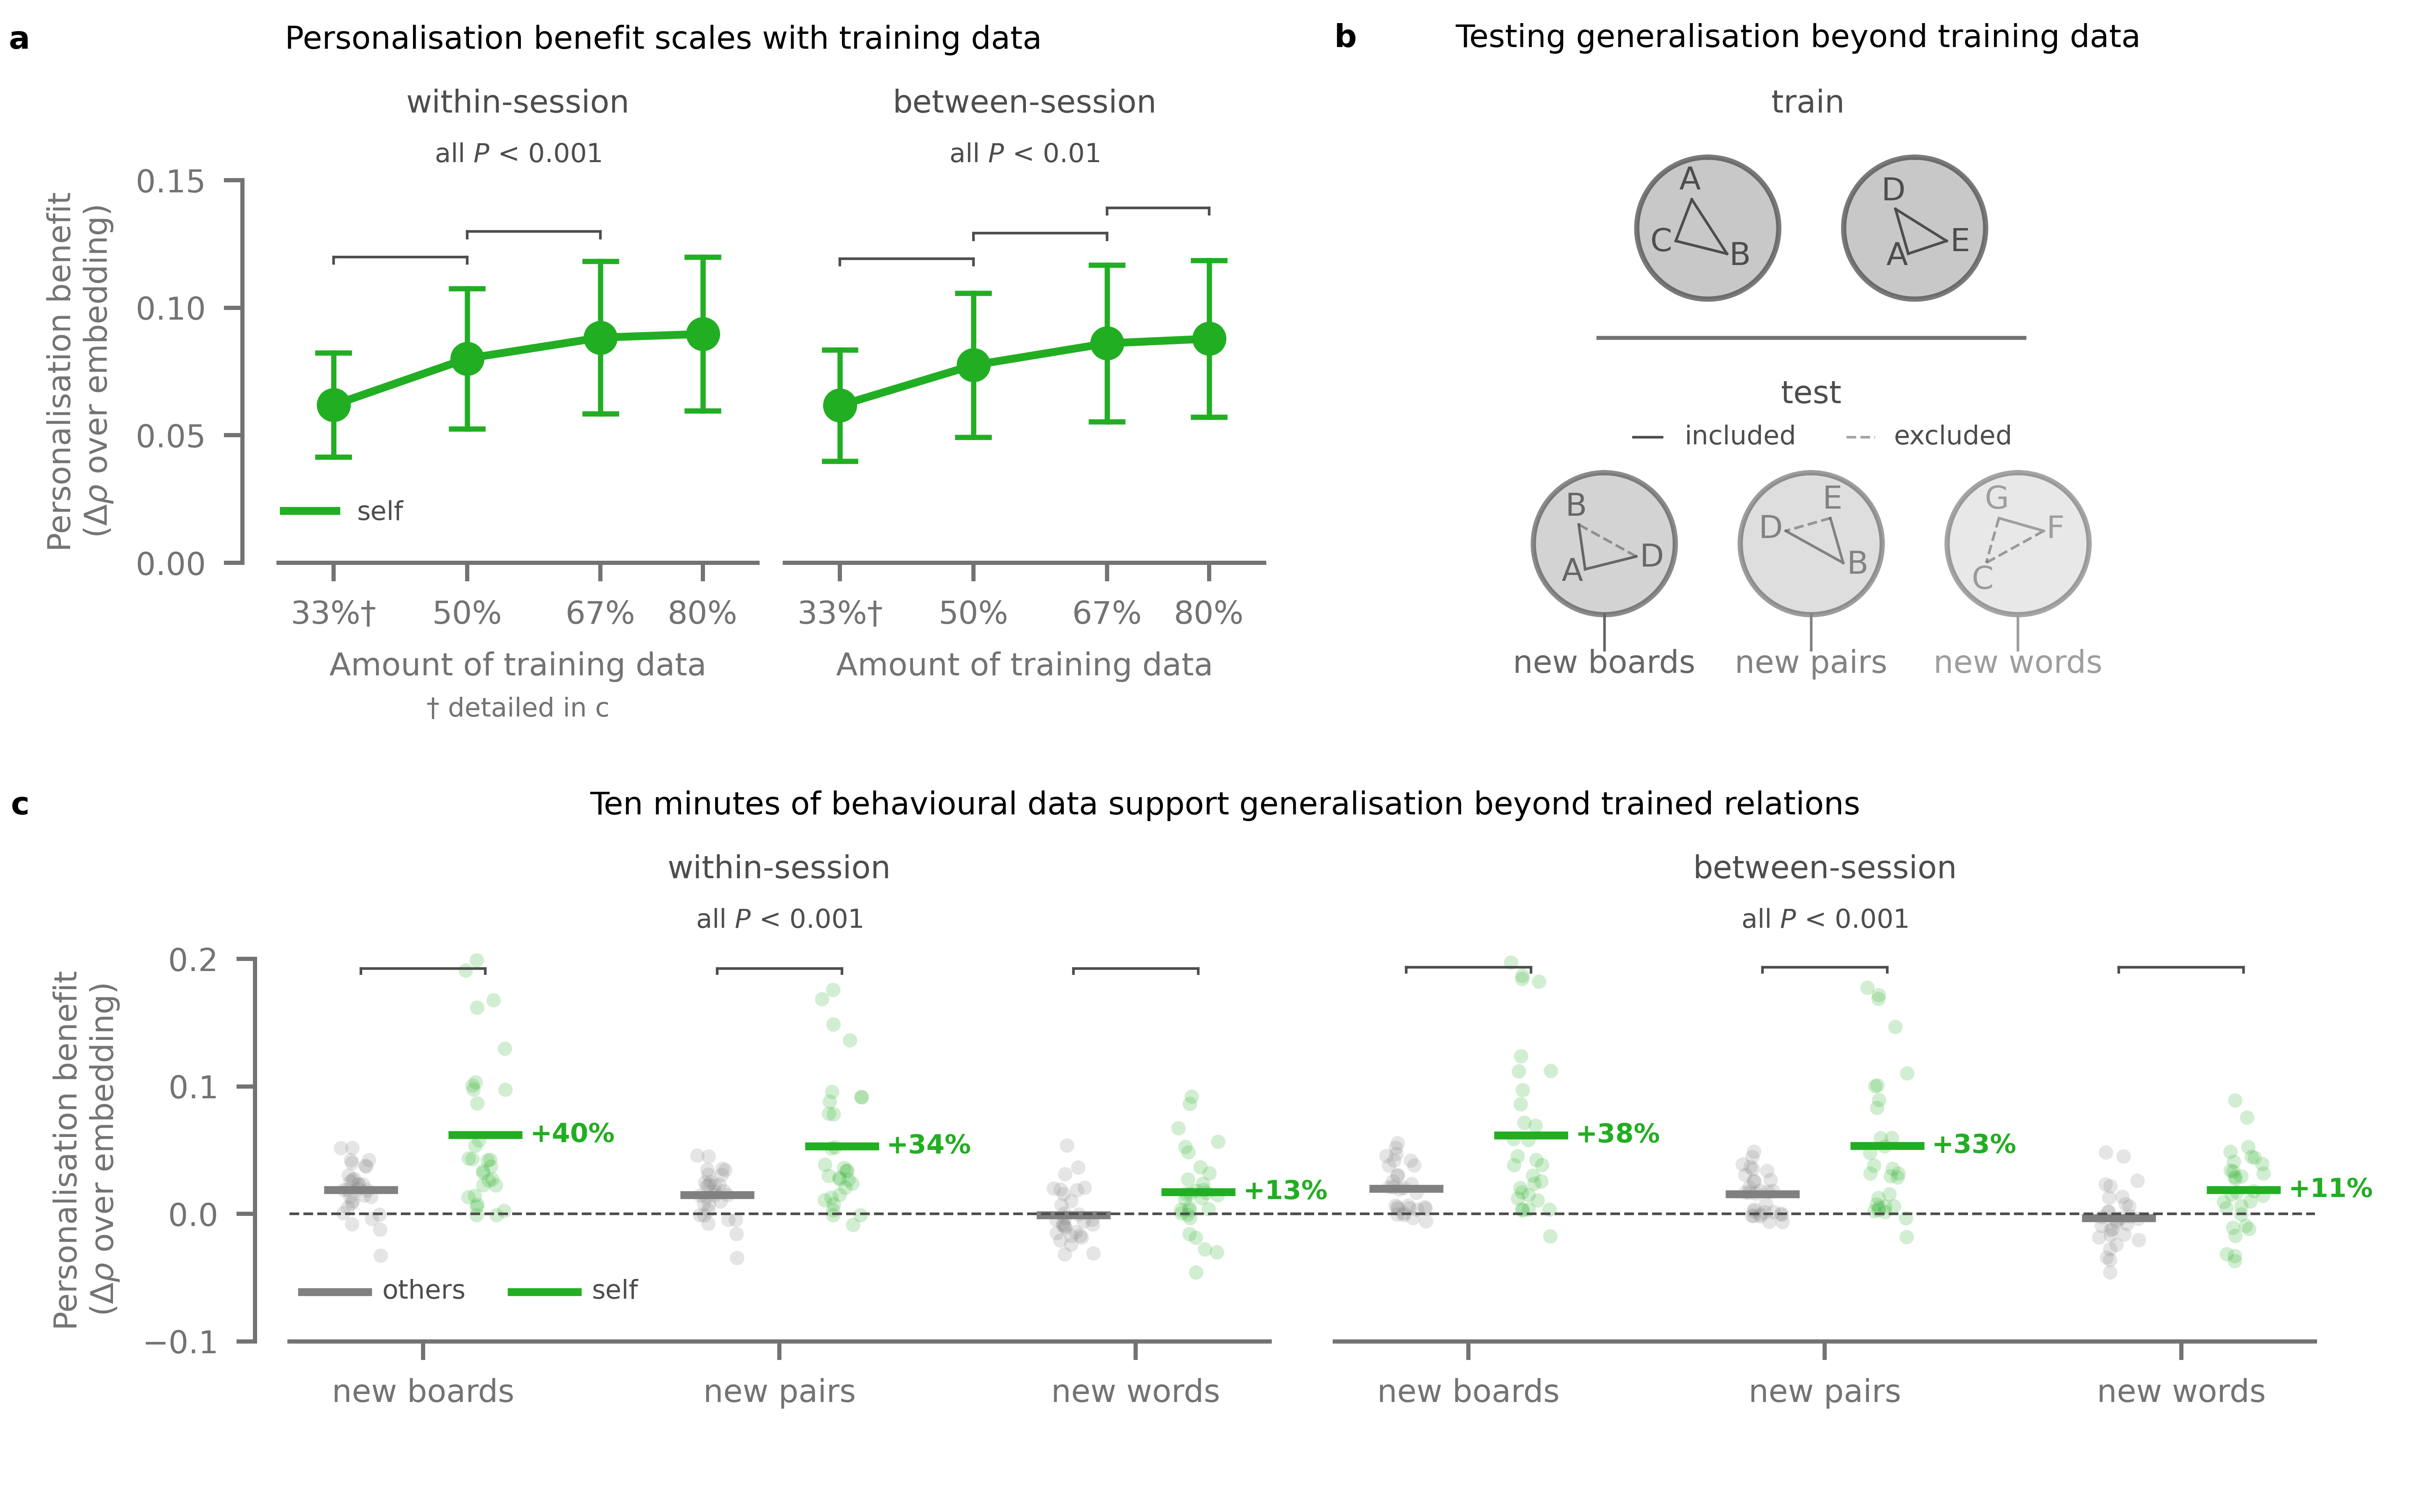
\includegraphics[width=0.9\paperwidth]{fig2.png}}
\caption{
\textbf{Individual adapters generalise beyond trained semantic relations.}
\textbf{a,} Benefits of personalised embeddings increased with the amount of behavioural data available for training. Adapters were trained on 33\%, 50\%, 67\% or 80\% of each participant's available data and tested on held-out boards. Benefits were reliable even in the sparsest training regime and increased monotonically but sublinearly as more boards were added. The 33\% condition is shown in detail in panel c. Points show means; error bars indicate 95\% confidence intervals.
\textbf{b,} Generalisation was tested under increasingly restrictive held-out conditions. Adapters were evaluated on held-out boards, held-out word pairs, and entirely held-out words.
\textbf{c,} Using only ten minutes of behavioural data, participant-specific adapters improved prediction beyond cross-participant adapters across all generalisation settings, indicating that the adapters learned individual transformations of semantic space rather than merely improving embeddings in a generic human-like direction. In each case, \textit{self} denotes the participant's own adapter and \textit{others} denotes the average cross-participant benefit from adapters trained on other participants. Dots indicate individual participants; horizontal bars indicate means. Statistical annotations indicate sign-flip permutation tests.
}\label{fig2}
\end{figure}

\subsection{Individual semantic structure can be estimated from sparse judgements}
If individual semantic differences reflect systematic tendencies across concepts, a limited sample of a person's judgements should already provide information about their judgements of other semantic relations. We therefore asked how readily this predictive structure could be recovered as behavioural observations accumulated. We trained adapters on progressively larger fractions of each participant's data, including 33\%, 50\%, 67\% and 80\%, and evaluated their predictions of held-out semantic judgements (see \nameref{scaling}).

Personalised embeddings improved embedding-participant fit even in the sparsest setting. When individual adapters were trained on only 33\% of the data, corresponding to five boards that participants completed in approximately ten minutes, personalisation already increased within-session prediction of held-out semantic geometry by 40\% relative to the original embedding model ($\Delta\rho = 0.062\pm0.004, P < 0.001$, sign-flip permutation test; Fig.~\ref{fig2}a). Scaling the amount of training data further improved performance: with 80\% of data available for training, personalised embeddings improved embedding-participant similarity by 58\% ($\Delta\rho = 0.090\pm0.002, P < 0.001$, sign-flip permutation test; Fig.~\ref{fig2}a).

Gains increased monotonically but sublinearly with additional training data. The largest improvement occurred when moving from the sparsest training regime to the intermediate amounts of data, whereas additional data produced progressively smaller gains (Fig.~\ref{fig2}a). This saturating pattern suggests that individual adapters rapidly capture a substantial component of participant-specific geometry, with diminishing returns as more behavioural data is added. The same pattern was observed when individual adapters were evaluated across sessions (Fig.~\ref{fig2}a), indicating that the personalisation benefit reflected temporally stable individual structure. Results were qualitatively consistent for embeddings derived from \texttt{T5} and \texttt{E5} (Supplementary Fig.~3). 

\subsection{Individual semantic differences generalise across concepts}
Training the model on only 33\% of the data allowed us to ask whether individual adapters learned individual semantic structure or merely fitted the observed behavioural relations. We considered three increasingly stringent forms of generalisation (see Fig.~\ref{fig2}b): first, we held out entire boards, requiring adapters to predict semantic geometries from arrangement contexts that were not used for training. Second, we held out individual word-pairs, requiring adapters to predict relations between words whose pairwise similarity had never been observed. Third, we held out entire words, requiring adapters to predict the semantic relations of words that were absent from the training data altogether (see \nameref{generalisation}).

First, individual adapters improved prediction of held-out board geometries relative to off-the-shelf embeddings and others by 40\% ($\Delta\rho = 0.062\pm0.004$) and 25\% ($\Delta\rho = 0.043\pm0.009$), respectively (all $P < 0.001$, sign-flip permutation tests; Fig.~\ref{fig2}c). This indicates that adapters did not simply reproduce the training arrangements, but learned individual-specific transformations that transferred to new arrangement contexts.

Second, for held-out pairs, personalised embeddings again showed benefits over off-the-shelf embeddings and others of 34\% ($\Delta\rho = 0.053\pm0.009$) and 22\% ($\Delta\rho = 0.038\pm0.008$), respectively (all $P < 0.001$, sign-flip permutation tests; Fig.~\ref{fig2}c). Thus, adapters learned a transformation of the semantic space that generalised beyond specific pairwise distances used for optimisation.

Finally, we evaluated the strongest form of generalisation by holding out entire words from training. In this setting, individual adapters have no information about held-out words or any of their relations. Any improvement therefore required the learned transformation to generalise from the geometry of trained words to new concepts within the embedding space. Individual adapters continued to show benefits over off-the-shelf embeddings and others of 13\% ($\Delta\rho = 0.017\pm0.006$) and 14\% ($\Delta\rho = 0.018\pm0.004$), respectively (all $P < 0.01$, sign-flip permutation tests; Fig.~\ref{fig2}c). This indicates that, even when coverage of the semantic space was sparse, individual adapters could nevertheless generalise to new concepts within the semantic space.

Together, these results show that individual adapters learned more than a set of memorised behavioural distances. With only ten minutes worth of sparse behavioural data, the individual adapters learned participant-specific transformations that transferred to new contexts, new geometric relations, and, most stringently, entirely new concepts within semantic space. Across all embeddings, participants' own adapters outperformed other participants' adapters for held-out boards and word pairs, both within and across sessions. For held-out words, this advantage was reliable across sessions for every embedding and within session for \texttt{GloVe} and contextualised \texttt{T5} (Fig.~\ref{fig2}c and Supplementary Fig.~4; see also replication in Supplementary Fig.~6).

\subsection{Sample characteristics predict embedding-human correspondence}
Having established that off-the-shelf embeddings capture individual semantic geometries only partially, we next asked whether the degree of embedding-human correspondence varied systematically across individuals. To reduce variation associated with national and linguistic context, we recruited an independent sample of $N = 303$ participants from the United States, all of whom were native speakers of English (see \nameref{participants}). Recruitment was balanced across self-reported age, gender, and ethnicity. Participants completed one session of the multiple-arrangement task, followed by a brief questionnaire assessing their interest in the semantic domains represented by the stimulus set (see \nameref{materials}). 

As in the initial sample, participants' judgements resembled their own held-out judgements more closely than either the original embedding or other participants' judgements (all $P < 0.001$, sign-flip permutation tests; Fig.~\ref{fig3}a). We therefore treated embedding-human similarity as an individual-level measure of how closely the embedding approximated each participant's semantic geometry, with lower values indicating greater embedding-human divergence. We tested whether this variation could be predicted from participants' age, gender, ethnicity, education, employment status and semantic-domain interests (Fig.~\ref{fig3}b). Because these characteristics are not statistically independent, we did not interpret individual regression coefficients in isolation. Instead, we evaluated whether the characteristics jointly predicted embedding-human similarity out of sample and subsequently quantified the incremental predictive contribution of each characteristic (see \nameref{embsub}).

\begin{figure}[H]%
\centering
\hspace*{0.0cm}
\noindent\makebox[\textwidth]{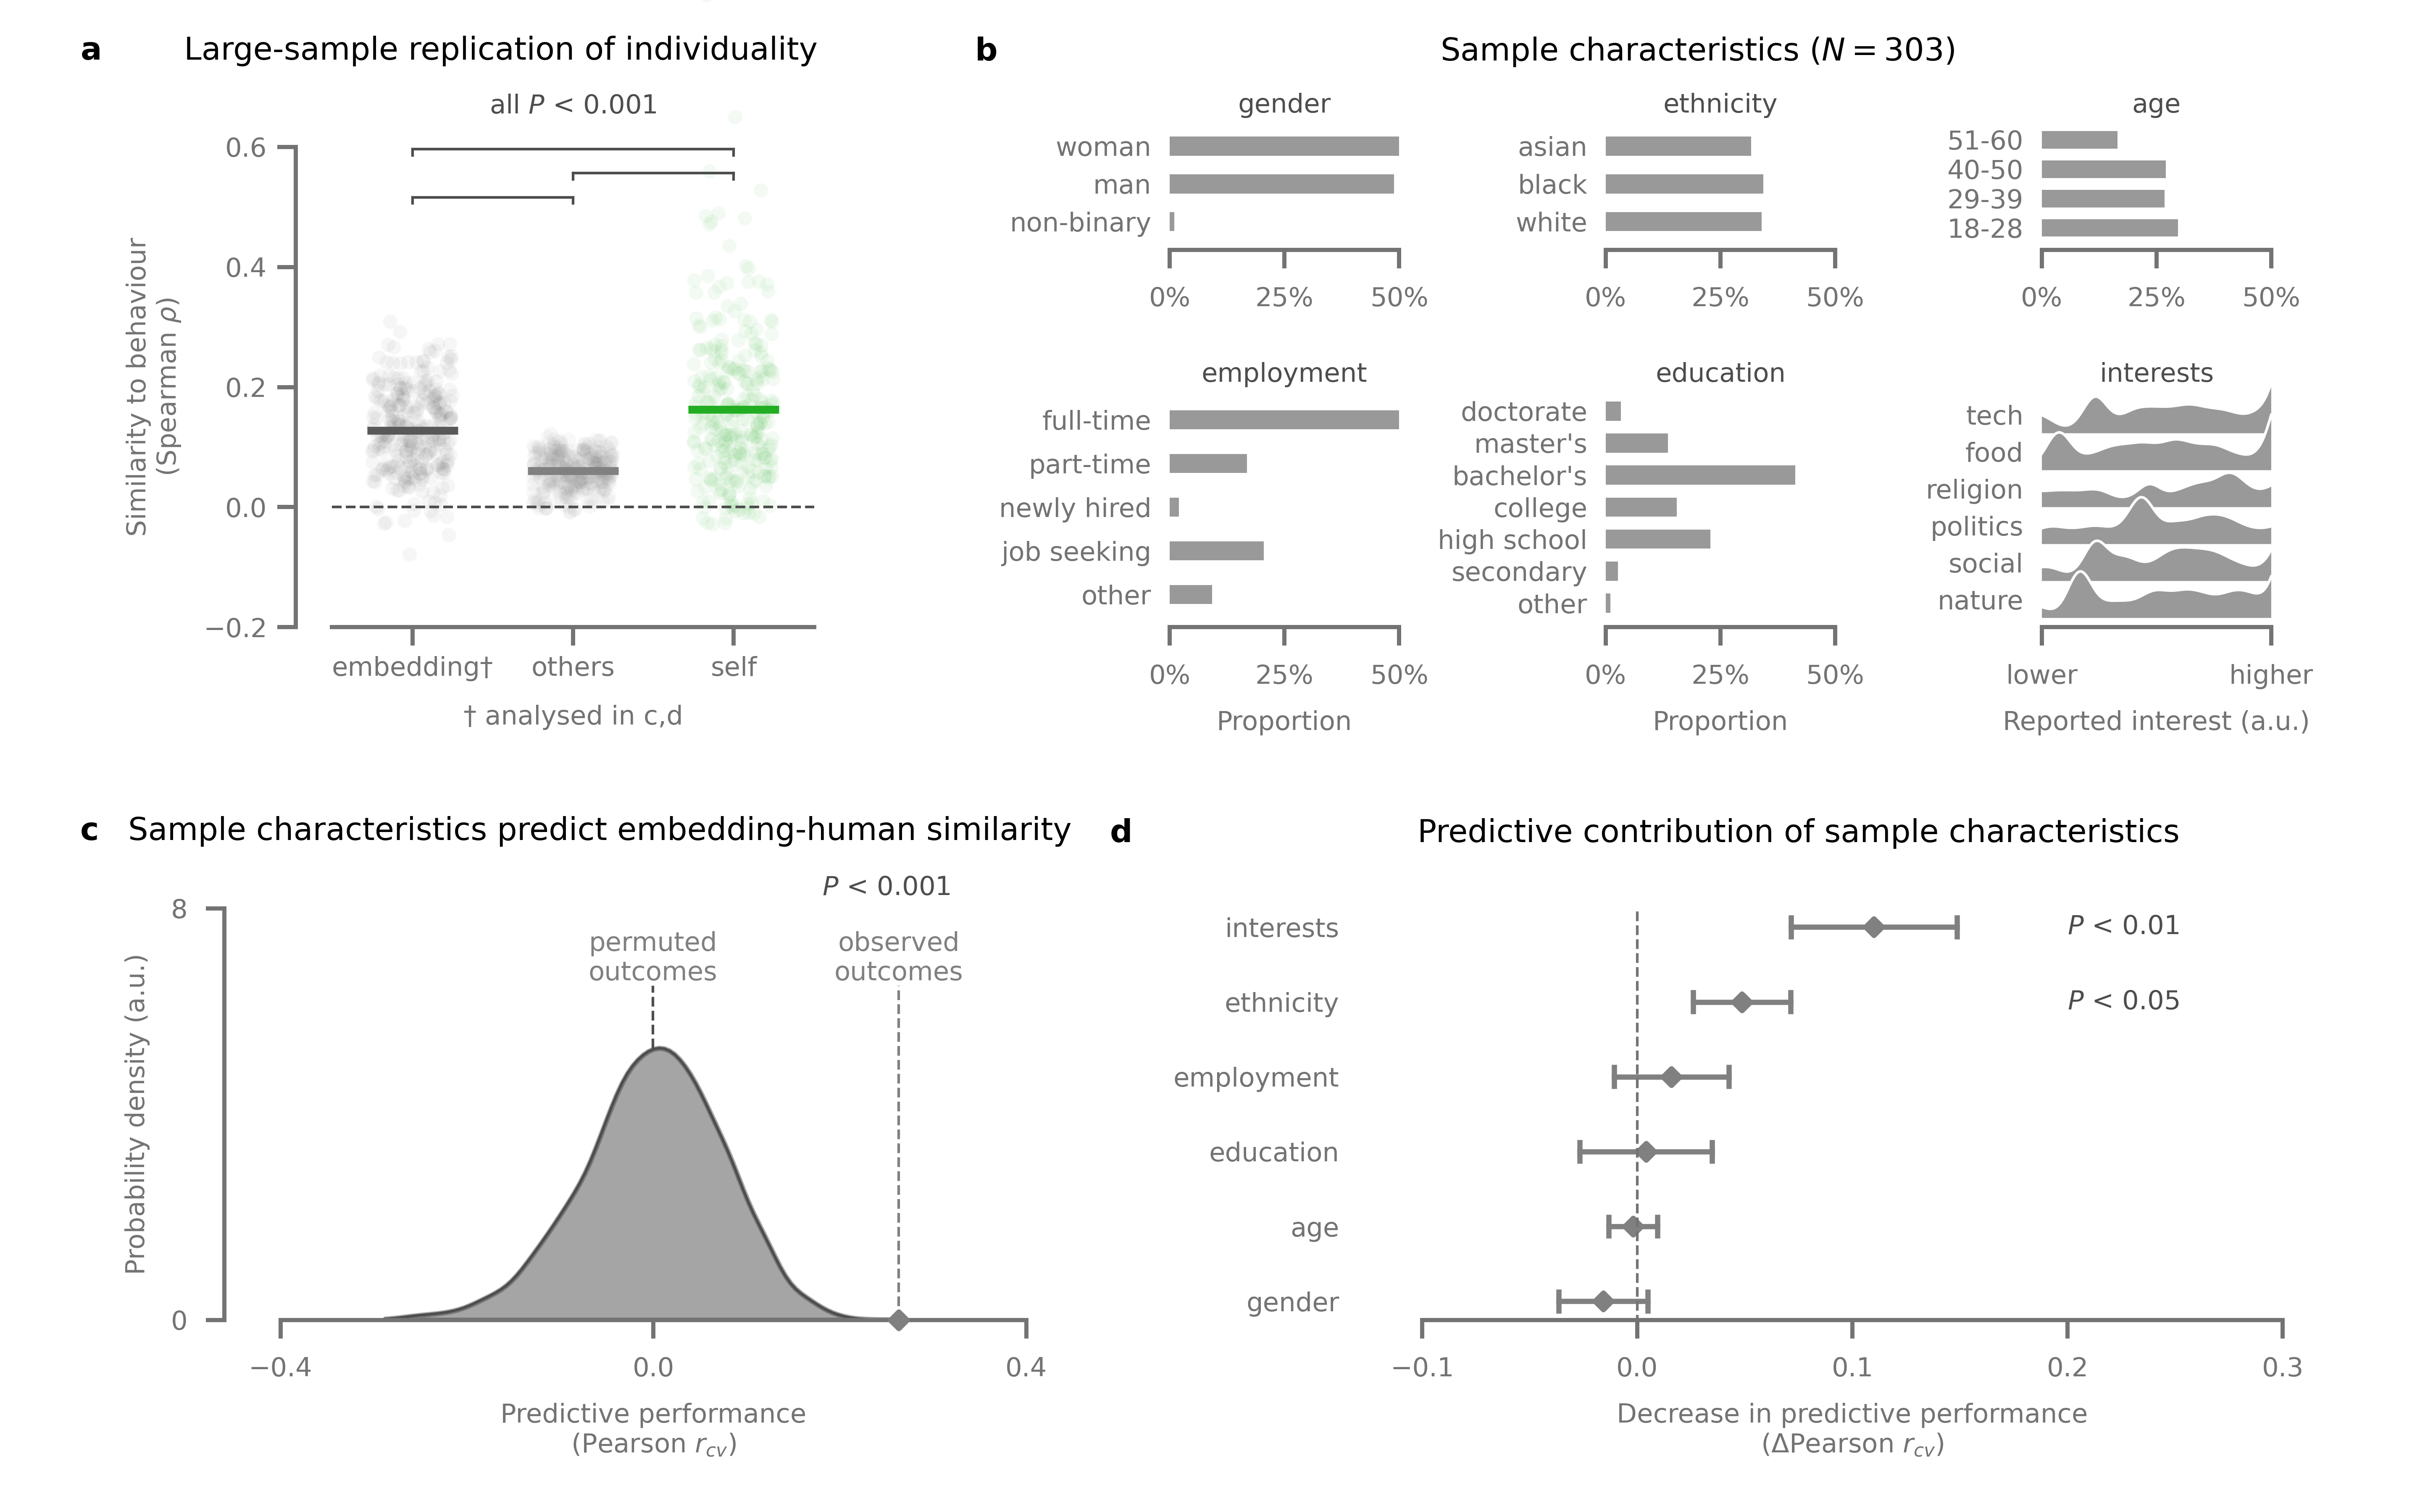
\includegraphics[width=0.9\paperwidth]{fig3.png}}
\caption{
\textbf{Sample characteristics predict embedding-human similarity.}
\textbf{a,} Large-sample replication of individual semantic  geometry in an independent sample of $N = 303$ participants. Each participant's semantic judgements were compared with the off-the-shelf embedding geometry, the semantic geometries of other participants, and their own held-out judgements. Participants were more similar to themselves than to either the embedding or other participants (all $P < 0.001$, sign-flip permutation tests). Points denote individual participants and horizontal lines indicate group means.
\textbf{b,} Composition of the sample across gender, ethnicity, age, employment and education. Bars show the proportion of participants in each characteristic category. Ridgeline plots show the distributions of self-reported interests, with higher values indicating greater reported interest.
\textbf{c,} Sample characteristics jointly predicted individual differences in embedding-human similarity. Predictive performance was evaluated out of sample as the Pearson correlation between observed and predicted embedding-human similarity. The grey distribution shows predictive performance under permutation of the outcome; the diamond and dashed line indicate the observed cross-validated performance ($P < 0.001$, permutation test).
\textbf{d,} Predictive contribution of individual sample characteristics, quantified as the decrease in cross-validated predictive performance ($\Delta$Pearson $r$) when the correspondence between each predictor block and participant identity was disrupted by permutation. Positive values therefore indicate that the characteristic contributed information beyond the remaining predictors. Interests and ethnicity made significant contributions to prediction ($P < 0.01$ and $P < 0.05$, respectively); error bars indicate 95\%-confidence intervals.
}\label{fig3}
\end{figure}

Sample characteristics jointly predicted agreement with the embedding in held-out participants ($r_{cv} = 0.264, P < 0.001$, permutation test; split-half noise ceiling $r = 0.917\pm0.015$; Fig.~\ref{fig3}c), demonstrating that correspondence between human and embedding geometries varied systematically across individuals. We assessed each characteristic's contribution by shuffling it across participants and measuring the resulting loss in predictive performance. Performance fell reliably when we shuffled semantic-domain interests ($\Delta r_{cv} = 0.110$) or ethnicity ($\Delta r_{cv} = 0.049$, all $P < 0.05$, permutation tests). No other characteristic produced a reliable decrease after Holm correction (Fig.~\ref{fig3}d). 

We repeated these analyses using \texttt{T5} and \texttt{E5} embeddings. Participant characteristics jointly predicted embedding-human similarity above chance across embeddings (all $P < 0.05$, permutation tests; Supplementary Fig.~5). Evidence for individual predictor contributions was less uniform. Ethnicity contributed significantly to prediction for \texttt{T5} and \textt{E5}, while interests also contributed significantly for \texttt{E5}. For contextualised \texttt{T5} embeddings, the estimated contributions of ethnicity and interests were positive, but did not survive correction for multiple comparisons. Thus, associations between sample characteristics and embedding-human correspondence generalised across embeddings, but contributions of specific characteristics were not consistently resolved (Supplementary Fig.~5).

Together, these results suggest that embedding-human similarity is not randomly distributed across participants, but is systematically related to demographic and experiential characteristics. Ethnicity was the most consistent predictor across embeddings, suggesting that variation in embedding-human correspondence reflects at least partly structured differences across individuals.

\subsection{Sample characteristics predict human-human similarity in semantic geometries}
The preceding analysis showed that correspondence between human semantic geometries and off-the-shelf embeddings varied systematically across participants. Variation in correspondence, however, does not itself establish whether participants that shared characteristics also deviated from the shared geometry in the same ways, or whether deviations reflect fully idiosyncratic differences. If individual semantic perception reflects variation in linguistic, social and experiential histories, then participants who share relevant characteristics should also exhibit more similar deviations from the semantic structure shared across the population.

We therefore asked whether similarities between participants' individual semantic deviations from their shared geometry could be predicted from their demographic and experiential characteristics. For each participant pair $(i, j)$, we first estimated the semantic structure shared by the remainder of the sample, excluding both members of the pair, and residualised each participant's semantic geometry with respect to this common reference. This procedure removed semantic structure shared across participants while retaining the participant-specific component of each geometry. We then quantified the correspondence between the two residual geometries using Spearman correlation, such that higher values indicated that two participants deviated from the shared semantic geometry in more similar ways (Fig.~\ref{fig4}a). We predicted these pairwise similarities from relationships between participants in age, gender, ethnicity, education, employment status and semantic-domain interests. We evaluated predictions on pairs for which both participants were held out from training to prevent leakage (see \nameref{subsub}). 

Sample characteristics jointly predicted similarity in participants' individual semantic deviations above chance ($r_{cv} = 0.027, P < 0.001$, permutation test; split-half noise ceiling $r = 0.513\pm0.015$; Fig.~\ref{fig4}b). Thus, although the predictive effect was small in magnitude, interindividual variation in semantic geometry was systematically structured by measurable characteristics of the participants. Shuffling ethnicity ($\Delta r_{cv} = 0.008$) or gender ($\Delta r_{cv} = 0.005$) labels reliably reduced predictive performance (all $P < 0.01$, permutation tests; Fig.~\ref{fig4}c). Semantic-domain interests showed a smaller effect that was significant before, but not after, correction for multiple comparisons ($\Delta r_{cv} = 0.002, P_{uncorrected} = 0.042, P = 0.166$), whereas no other characteristic showed a reliable contribution. 

\begin{figure}[H]%
\centering
\hspace*{0.0cm}
\noindent\makebox[\textwidth]{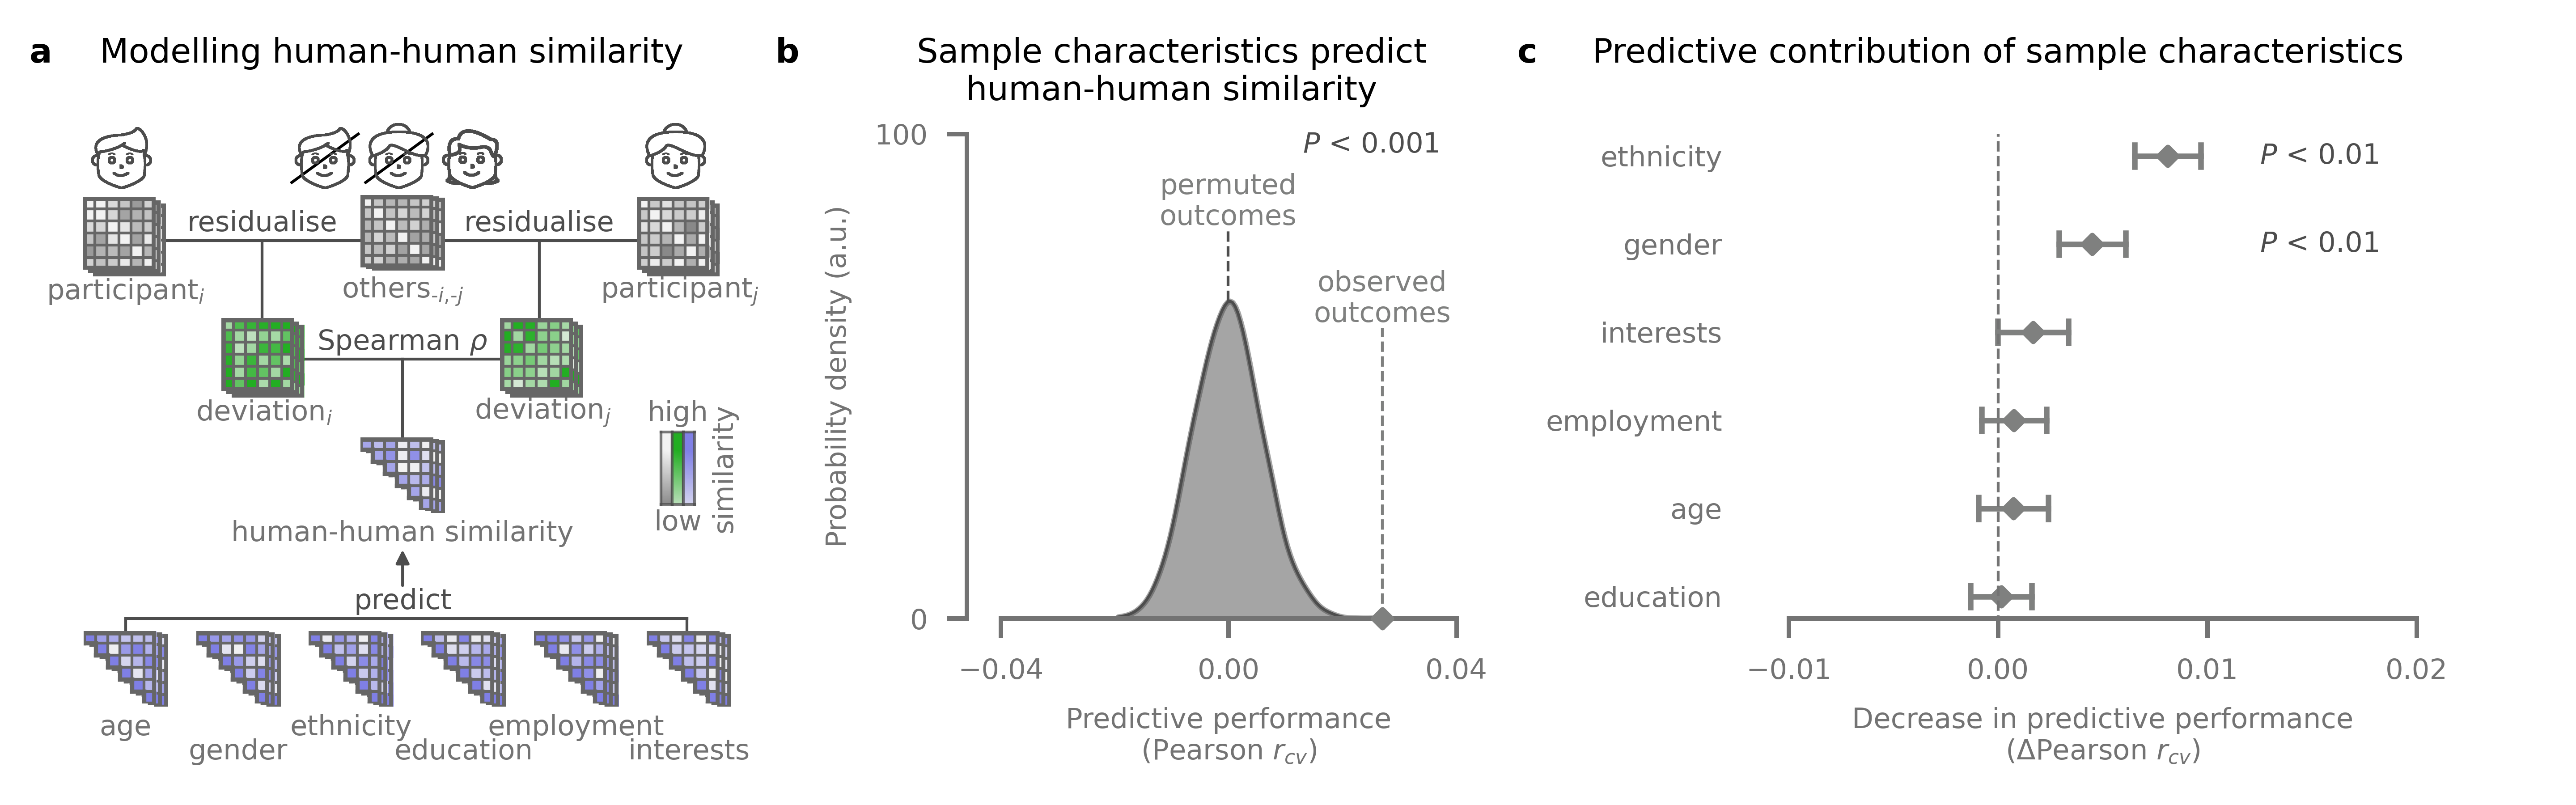
\includegraphics[width=0.9\paperwidth]{fig4.png}}
\caption{
\textbf{Sample characteristics predict human-human similarity in semantic geometries.}
\textbf{a,} Schematic of the analysis. For each participant pair $(i,j)$, the semantic geometry of each participant was residualised with respect to the aggregate geometry of all remaining participants, excluding both members of the pair ($\mathrm{others}_{-i,-j}$). Spearman correlations between the resulting participant-specific deviation matrices quantified pairwise correspondence in deviations from the shared semantic geometry. Pairwise similarities in these deviations were then predicted from participants' relationships in age, gender, ethnicity, education, employment, and interests.
\textbf{b,} Cross-validated predictive performance of the full model. Sample characteristics predicted human-human similarity in deviations from their shared geometry above chance, assessed against a permutation distribution obtained by shuffling the participant identities ($P < 0.001$, permutation test). The diamond indicates the observed cross-validated Pearson correlation.
\textbf{c,} Predictive contribution of individual sample characteristics, quantified as the decrease in cross-validated performance ($\Delta$Pearson $r$) when participant identities within each characteristic were permuted before dyad computation and model fitting. Ethnicity and gender made the largest statistically reliable contribution to prediction (all $P < 0.01$, permutation tests).
}\label{fig4}
\end{figure}

Together, these results indicate that individual semantic geometries are not fully idiosyncratic in a narrow participant-specific sense. Rather, some of the ways in which individuals deviate from the semantic structure shared across the sample are themselves systematically shared between participants with similar characteristics. Ethnicity and gender provided the clearest evidence for such structure in the present sample. 

\subsection{Shared and individual semantic divergences reflect non-linear deformations}
Having established that participants exhibit structured individual differences from their shared geometry and each other, we next asked what kinds of transformations capture these divergences. One possibility is that they primarily reflect global transformations, such as reweighting semantic dimensions\cite{Mirman2017,Kallens2025}. Alternatively, they may require transformations that vary across semantic space, allowing different regions to deform in different ways\cite{Johns2024}. To distinguish these possibilities, we compared personalisation models with linear and non-linear transformations.

We first replicated out-of-sample generalisation with our original personalisation model in the larger sample, using approximately ten minutes of behavioural data per participant (all $P < 0.001$, sign-flip permutation tests).  We then compared parameter-matched linear and non-linear personalisation models, each comprising shared and participant-specific transformations (see \nameref{nonlinear}). Linear models applied a single learned linear map throughout the embedding space, whereas non-linear models allowed the mapping to vary across semantic regions. We evaluated whether the flexibility afforded by non-linear deformations improved out-of-sample prediction of shared and individual semantic structure (see Fig.~\ref{fig5}a). Predictions were evaluated for held-out boards, pairs, and words (see Fig.~\ref{fig2}b).

Non-linear personalisation improved prediction relative to off-the-shelf embeddings by approximately 30\%, 28\% and 13\% for new boards, pairs and words, respectively ($\Delta\rho = 0.040\pm0.003$, $0.040\pm0.003$, $0.020\pm0.002$; all $P < 0.001$; sign-flip permutation tests; Fig.~\ref{fig5}a). Predictions were also more accurate using participants' own transformations than transformations fitted to other participants, with corresponding improvements of 16\%, 14\% and 6\% ($\Delta\rho = 0.020\pm0.002$, $0.020\pm0.002$, $0.01\pm0.001$, all $P < 0.001$; sign-flip permutation tests; Fig.~\ref{fig5}a), demonstrating a person-specific benefit.

Conversely, linear transformations yielded gains of less than 1\% over off-the-shelf embeddings across all three forms of generalisation. Gains were significant for new boards and pairs (both $P < 0.001$), but not new words ($P = 0.77$; sign-flip permutation tests; see Fig.~\ref{fig5}a). Critically, non-linear transformations consistently outperformed parameter-matched linear transformations (new boards: $\Delta\rho = 0.040\pm0.003$; new pairs: $0.040\pm0.03$; new words: $0.020\pm0.001$; all $P < 0.001$; sign-flip permutation tests; Fig.~\ref{fig5}a). We replicated these findings using \texttt{T5} and \texttt{E5} embeddings (Supplementary Fig.~6). Thus, allowing the mapping to vary across embedding space improved generalisation beyond that achieved by a single global linear transformation.

\begin{figure}[H]%
\centering
\hspace*{0.0cm}
\noindent\makebox[\textwidth]{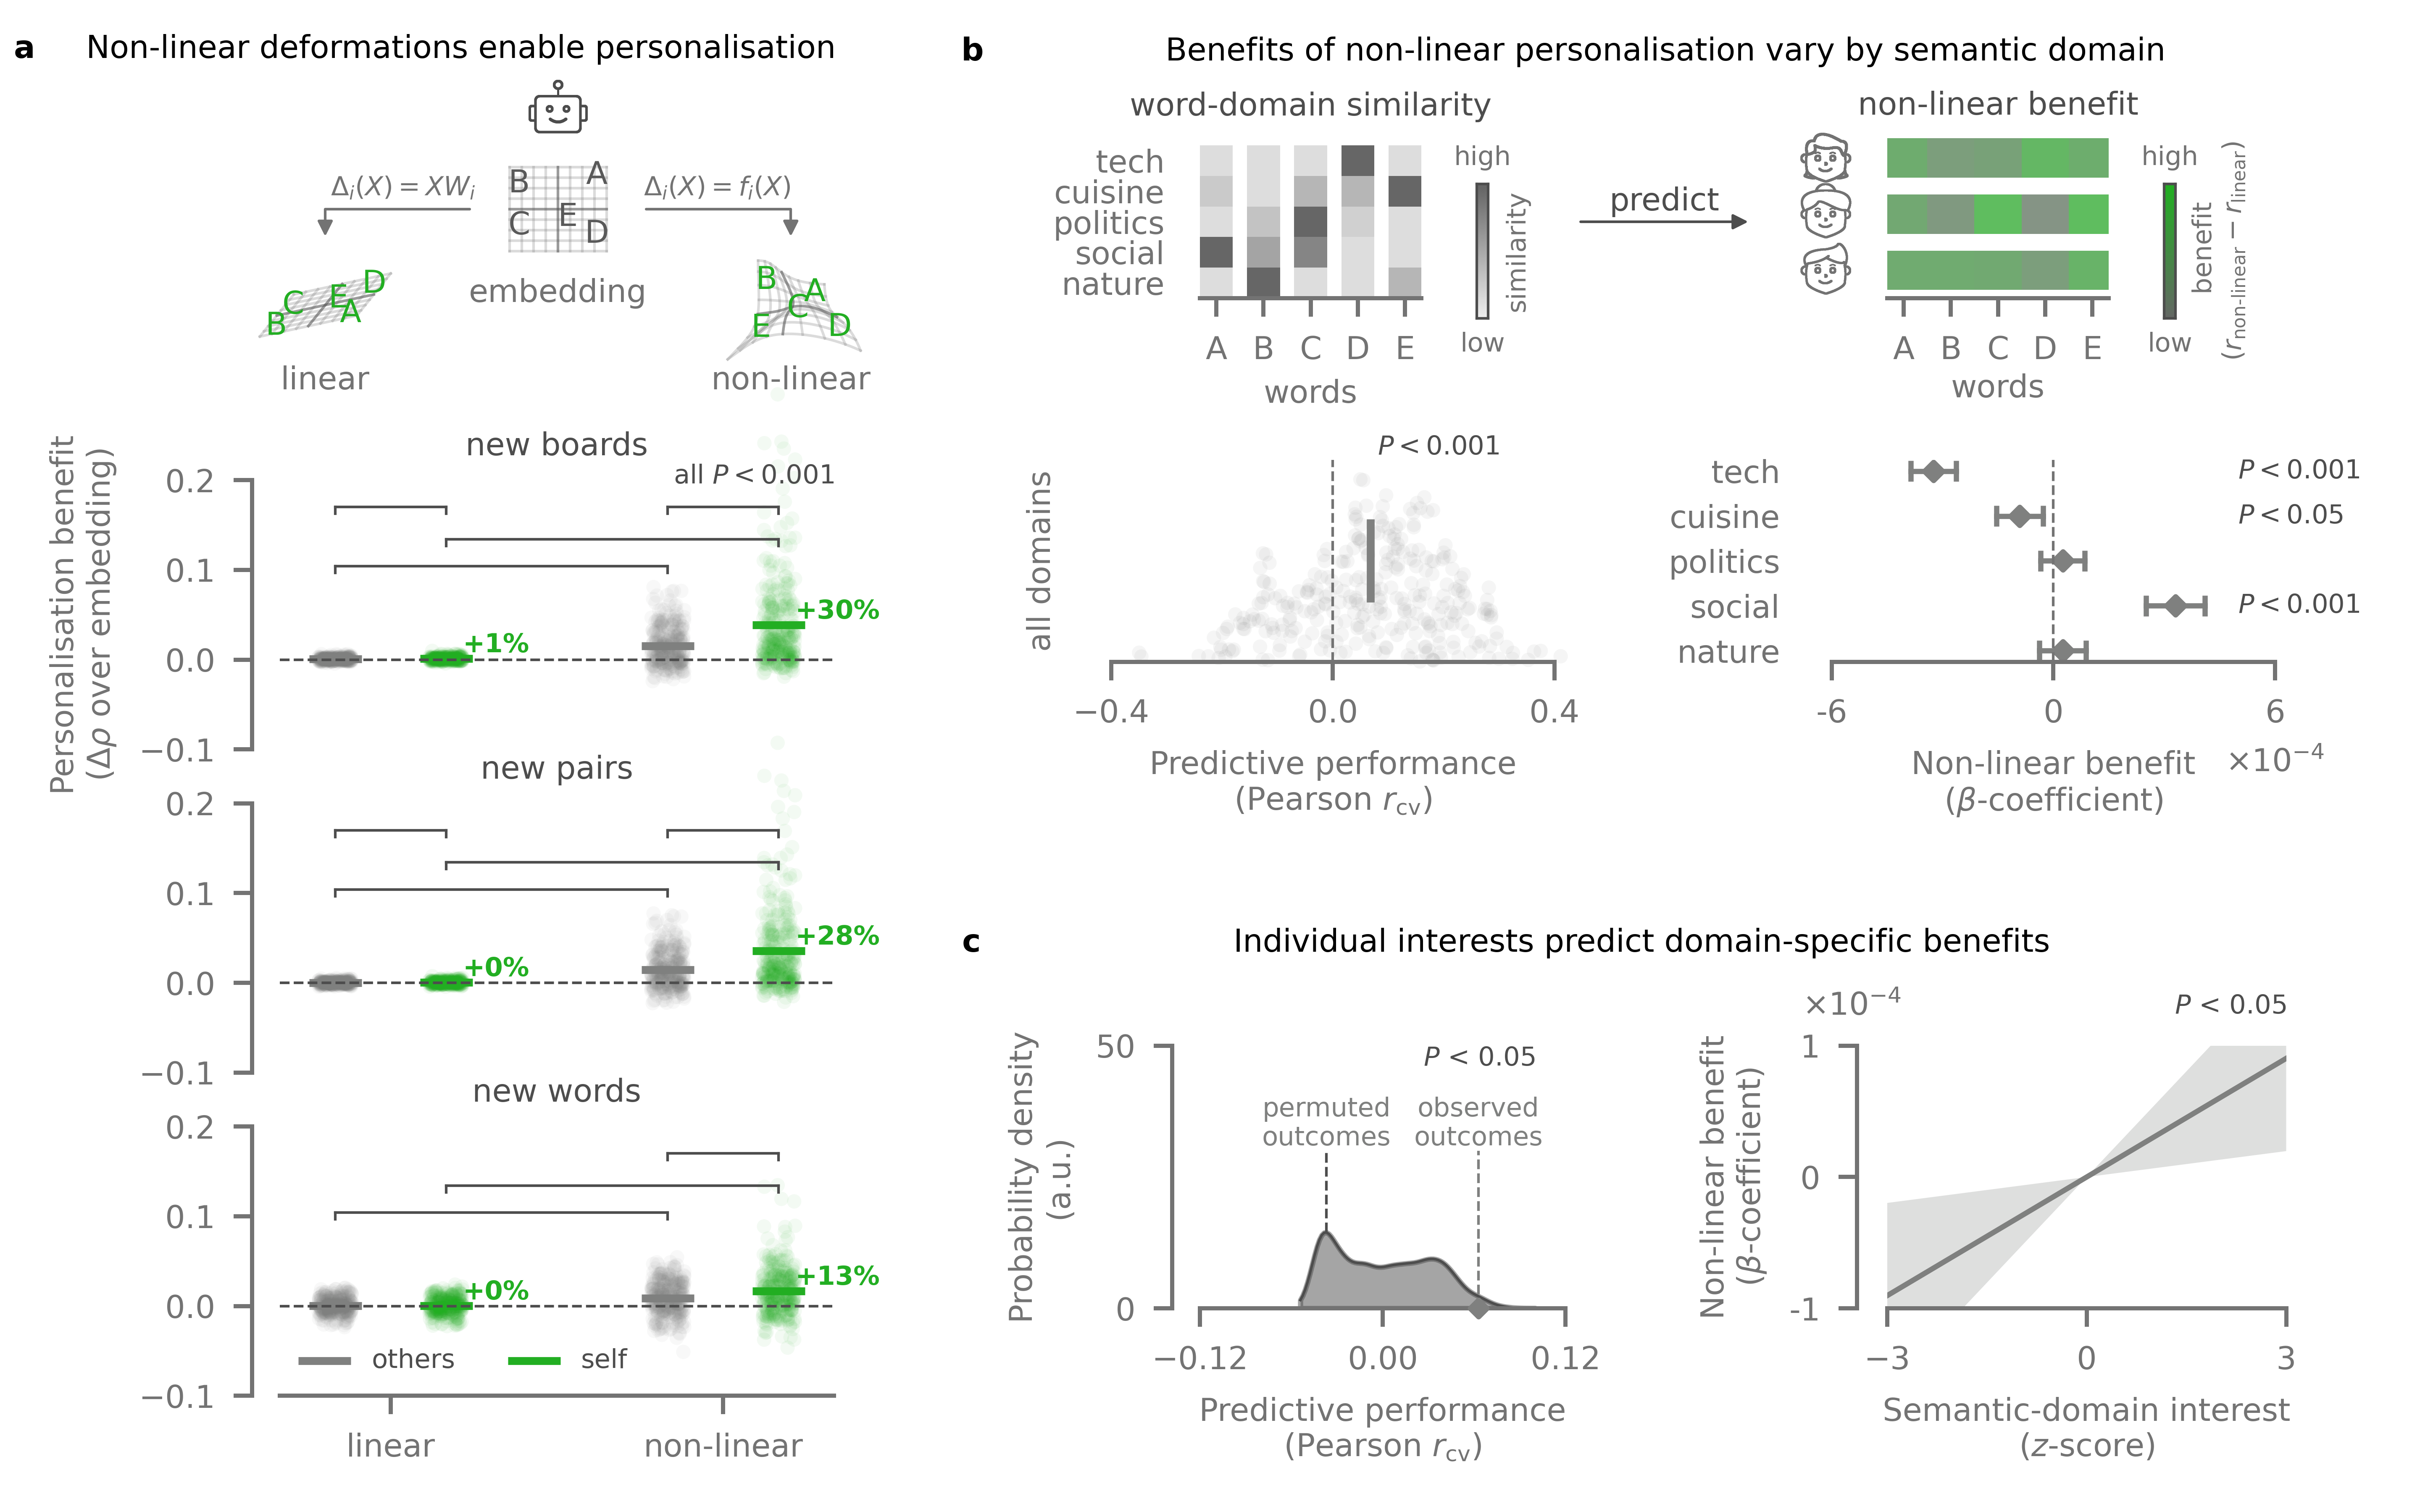
\includegraphics[width=0.9\paperwidth]{fig5.png}}
\caption{
\textbf{Non-linear personalisation improves semantic prediction, with benefits varying by domain and individual interest.}
\textbf{a,} Parameter-matched linear and non-linear transformations were compared in their ability to predict held-out semantic geometries. Schematics illustrate a global linear transformation and a non-linear deformation of the embedding space. Plots show improvements over off-the-shelf embeddings ($\Delta\rho$, Spearman correlation) for held-out boards, pairs, and words. Predictions used transformations fitted to the target participant (self, green) or other participants (others, grey). Points represent participants; horizontal bars indicate means. Percentages indicate relative improvements in mean self prediction over the off-the-shelf embedding. Brackets indicate pairwise comparisons.
\textbf{b,} Semantic-domain similarity predicts the word-level advantage of non-linear over linear personalisation. For each participant, word-level benefits were modelled using similarities to five semantic domains. Left, predictive performance on held-out words (Pearson $r_{\mathrm{cv}}$); points represent participants and the vertical bar indicates the mean. Right, coefficients from the full model indicate the direction and magnitude of associations between domain similarity and non-linear benefit.
\textbf{c,} Reported interests predict individual differences in domain-specific non-linear benefits. Left, observed cross-validated prediction of participant-specific domain coefficients, evaluated in held-out participants, relative to a null distribution generated by permuting participant identities while preserving interest profiles. Right, model-predicted domain coefficients as a function of standardised interest in the corresponding domain.
}\label{fig5}
\end{figure}

\subsection{Non-linear personalisation benefits vary by semantic domain and individual interest}
Next, we asked where in semantic space the additional flexibility of non-linear over linear transformations was most beneficial. Identifying systematic variation across semantic domains could reveal which kinds of meaning are better captured by local non-linear deformations. Moreover, if these benefits are related to personal relevance, their distribution across domains may vary with individuals' interests. We therefore first tested whether semantic-domain similarity predicted word-level benefits of non-linear over linear transformations. For each participant, we modelled word-level differences in predictive performance as a function of word similarity to five semantic domains: technology, cuisine, politics, social interactions and nature. Models were evaluated on held-out words (see \nameref{nonlinear-words}).

Word-level semantic-domain similarity predicted non-linear benefits above chance ($r_{cv} = 0.068\pm0.008, P < 0.001$; sign-flip permutation test; Fig.~\ref{fig5}b). Greater similarity to the social domain was associated with larger non-linear benefits ($\beta = 3.31\times10^{-4}\pm4.06\times10^{-5}, P < 0.001$), whereas similarity to technology and cuisine was associated with smaller benefits (technology: $\beta = -3.24\times10^{-4}\pm3.14\times10^{-5}, P < 0.001$; cuisine: $\beta = -9.10\times10^{-5}\pm3.25\times10^{-5}, P < 0.05$), and associations with politics and nature were not significant (both $P > 0.05$, sign-flip permutation tests; Fig.~\ref{fig5}b). Domain similarity also predicted benefits for held-out words with contextualised \texttt{T5} and \texttt{E5}, whereas predictions did not reach significance for decontextualised \texttt{T5} (Supplementary Fig.~6). Across the three embeddings for which domain similarity predicted held-out benefits, similarity to the social domain was associated with the largest benefits (Fig.~\ref{fig5}c, Supplementary Fig.~6). Together, these results indicate that the benefit of non-linear personalisation varied systematically with semantic content.

We next tested whether participants' reported interests predicted the domain coefficients estimated above. Interests weakly predicted domain-specific coefficients in held-out participants ($r_{cv} = 0.062\pm0.001, P < 0.05$; permutation test; Fig.~\ref{fig5}c). Greater interest in a domain was associated with a more positive coefficient for that domain ($\beta = 2.98\times10^{-5}\pm1.83\times10{-7}, P < 0.05$; permutation test; Fig.~\ref{fig5}c). We replicated these findings using \texttt{T5} and \texttt{E5} embeddings (Supplementary Fig.~6). This suggests that non-linear benefits were greater for words related to semantic domains that participants expressed interest in.

\subsection{Affective and interoceptive word features predict non-linear personalisation benefits}
The domain-specific patterns above raise the question of which properties of words predict the benefit of non-linear personalisation. Semantic domains naturally encompass multiple dimensions of meaning, including sensory, affective and social associations, as well as differences in familiarity and related lexical properties. Examining these features could therefore identify more specific properties associated with the advantage of non-linear over linear transformations. For each participant, we modelled word-level non-linear benefits using 17 normative word features spanning social, sensory, affective and lexical properties, and evaluated predictions on held-out words (see \nameref{nonlinear-words}; Fig.~\ref{fig6}a).

\begin{figure}[H]%
\centering
\hspace*{0.0cm}
\noindent\makebox[\textwidth]{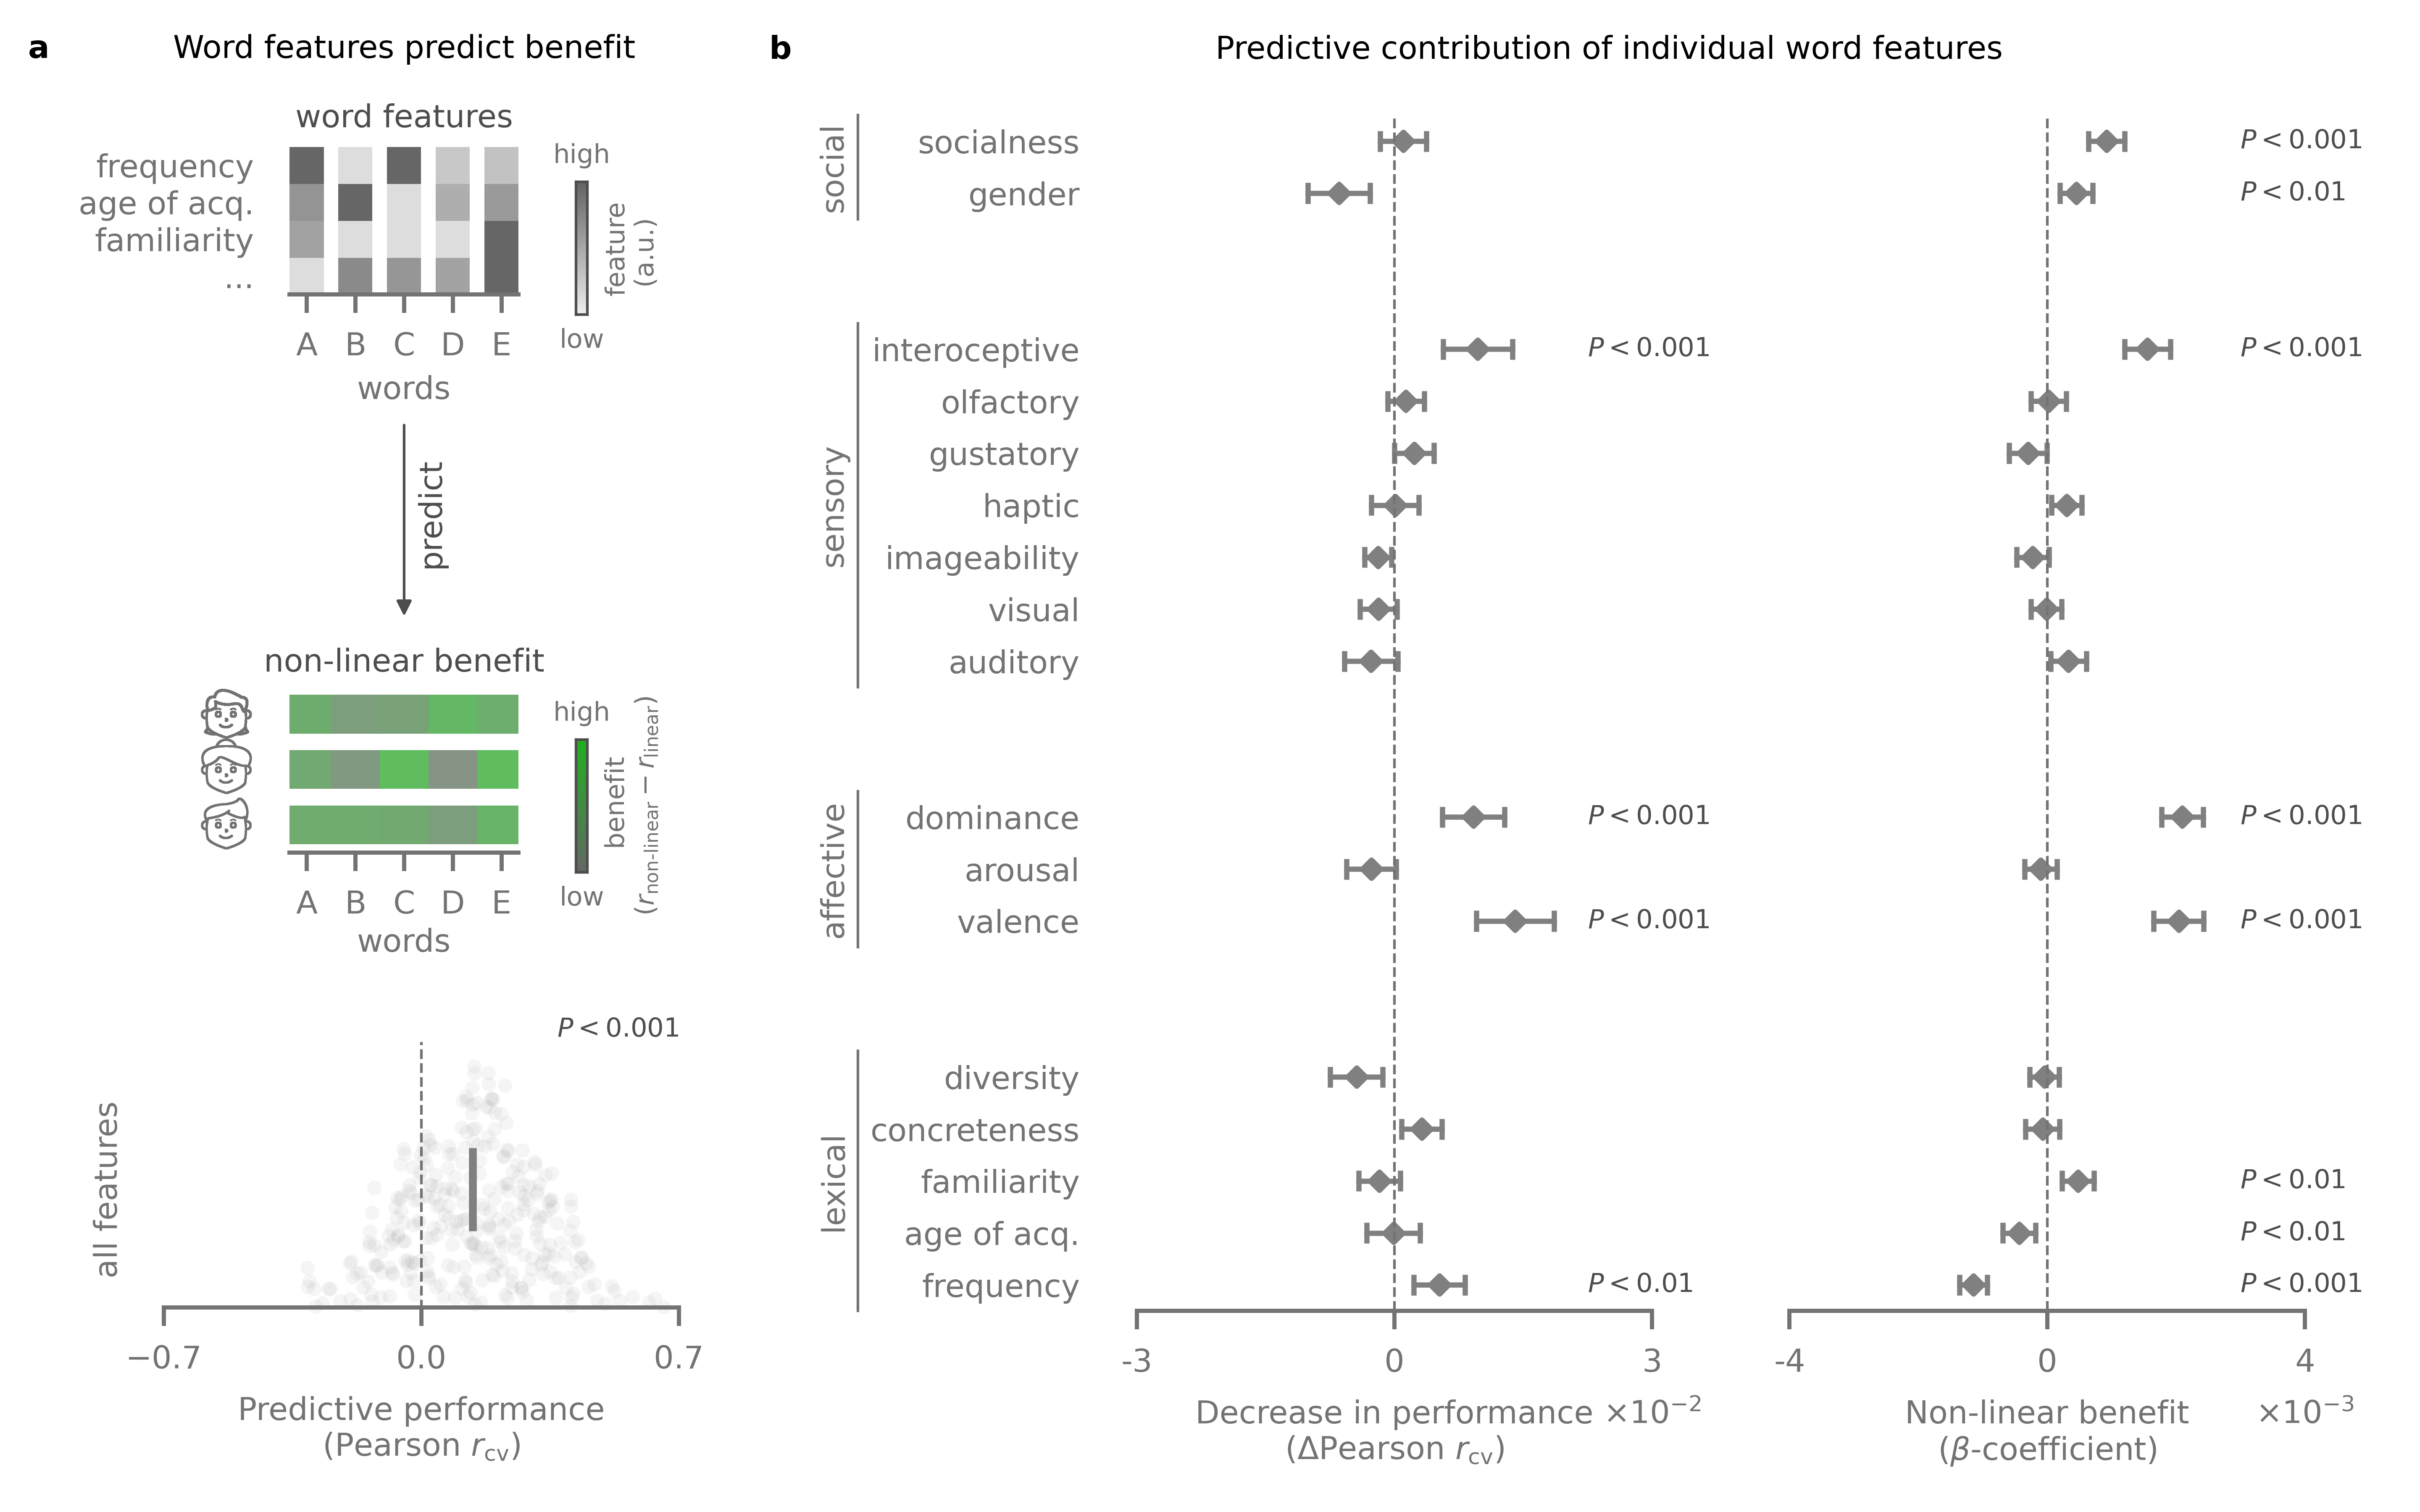
\includegraphics[width=0.9\paperwidth]{fig6.png}}
\caption{
\textbf{Interoceptive, affective and lexical word properties predict non-linear personalisation benefits.}
\textbf{a,} For each participant, 17 normative word features were used to predict the word-level advantage of non-linear over linear personalisation of \texttt{GloVe} embeddings ($\Delta$Spearman $\rho$). Models were evaluated on held-out words. The schematic illustrates the predictors and participant-specific outcomes; the lower plot shows cross-validated predictive performance (Pearson $r_{cv}$). Points represent participants and the vertical bar indicates the mean. 
\textbf{b,} Left, incremental predictive contribution of each feature, quantified as the decrease in cross-validated performance when that feature was omitted and the model refitted. Positive values indicate that including the feature improved prediction. Right, coefficients from the full model indicate the direction and magnitude of associations with non-linear benefit, conditional on the remaining features. Diamonds denote means across participants; error bars indicate 95\%-confidence intervals. Interoceptive strength, dominance, valence, and frequency contributed predictive information, with larger benefits associated with stronger interoceptive associations, higher dominance and more positive valence, and smaller benefits associated with higher frequency. Statistical annotations indicate sign-flip permutation tests, with Holm correction across features applied separately to predictive contributions and coefficients.
}\label{fig6}
\end{figure}

Word features predicted non-linear benefits above chance ($r_{cv} = 0.139\pm0.011, P < 0.001$, sign-flip permutation test; Fig.~\ref{fig6}a). To assess the predictive contribution of each feature, we compared the full model with reduced models that omitted one predictor at a time. This revealed unique predictive information provided by interoceptive strength, dominance, valence, and frequency (all $P < 0.01$; sign-flip permutation tests; Fig.~\ref{fig6}b). Concreteness appeared to add predictive information before but not after corrections for multiple comparisons ($P_{\text{uncorrected}} = 0.004$, $P_{\text{Holm}} = 0.058$). Coefficients from the full model indicated larger non-linear benefits for words with stronger interoceptive associations, higher dominance and higher valence ratings as well as a smaller benefit for more frequent words (all $P < 0.001$; sign-flip permutation tests; Fig.~\ref{fig6}b). Additionally, positive relationships with non-linear benefits were observed for socialness ($P < 0.001$), genderedness ($P < 0.01$) and familiarity ($P < 0.01$) as well as a negative association with age of acquisition ($P < 0.05$). However, removing these features did not significantly reduce predictive performance, indicating that their coefficient associations did not translate into detectable predictive value.

We repeated these analyses using (de-)contextualised \texttt{T5} and \texttt{E5} embeddings. Word features predicted non-linear personalisation benefits for contextualised \texttt{T5} and \texttt{E5} (all $P < 0.001$, sign-flip permutation tests; Supplementary Fig.~7). In both embeddings, interoceptive strength, dominance and valence added reliable predictive information (all $P < 0.05$, sign-flip permutation tests). Consistent with our main findings, words with stronger interoceptive associations, higher dominance and higher valence showed larger benefits from non-linear personalisation (all $P < 0.05$, sign-flip permutation tests). Gustatory strength additionally contributed predictive information for contextualised \texttt{T5}, whereas the contribution of frequency observed for \texttt{GloVe} did not survive correction in either embedding. For decontextualised \texttt{T5}, neither the full model nor any individual feature's incremental contribution reached significance.

Together, these analyses identify interoceptive and affective word properties as recurring predictors of the advantage of non-linear over linear personalisation across three embedding representations. Contributions from other word properties were less consistent, and prediction from normative features did not generalise to all embeddings.

\section{Discussion}\label{discussion}
Here we asked whether individual semantic judgements contain reliable structure that extends beyond the relations directly measured. Across two studies (total $N = 333$), participants' judgements were reliably more similar to their own held-out judgements than to embeddings or to other participants' judgements. In the initial cohort, adapting embeddings with approximately ten minutes of behavioural data improved prediction of held-out arrangements by about 40\% relative to the off-the-shelf embedding and by 25\% relative to adapters fitted to other participants, with smaller but reliable benefits for unobserved word pairs and words (Fig.~\ref{fig2}). In the larger sample, participant characteristics, chiefly ethnicity, interests, and gender, predicted alignment between embeddings and individual geometries and, more weakly, the similarity of individuals' deviations from the group geometry (Figs.~\ref{fig3}-\ref{fig4}). Only non-linear transformations of the embedding space yielded appreciable personalisation benefits, and these benefits varied with semantic content, personal interests, and affective and interoceptive word properties (Figs.~\ref{fig5}-\ref{fig6}).

Together, these findings support three conclusions about how individuals' semantic judgements are organised. First, individual differences are stable and systematic rather than noise: a person's departures from the embedding persist across sessions and extend across concepts, such that their judgements about some words inform predictions about others. These departures are partly shared across people, as adapters trained on other participants also improved prediction, and partly person-specific, as a person's own adapter performed better still. Second, individual departures are partly structured by demographic and experiential characteristics, in that people who share them tend to deviate from the group geometry in more similar ways, although this structure is weak relative to the reliable individual variance. Third, the transformations that capture these departures are non-linear in embedding space, consistent with conceptually local rather than global changes. Their benefit was largest for words in the social domain and words with strong interoceptive and affective associations, and tended to be larger in domains in which participants reported greater interest.

Previous work has shown substantial individual differences in meaning across several measures: similarity and feature judgements, semantic spaces derived from individuals' own language use, and neural representations\cite{Marti2023,Johns2024,Guitard2027,Charest2014,Wang2021}. We extend these findings by showing that these differences are internally structured. Sparse observations of a person's semantic judgements predict their judgements of semantic relations that were not used for training. The benefit for held-out words is particularly informative, because adapters had access to those words' original embeddings, but no participant-specific judgements involving them. Its predictions therefore depended on regularities connecting observed and unobserved parts of the embedding space. This indicates that individual differences contain sufficient structure for information about one set of concepts to inform predictions about another, and that this structure is learnable from a few minutes of behavioural data.

Yet, individuality need not imply that each person possesses an entirely separate semantic system. Adapters trained on other participants also improved predictions, indicating that adaptation captured departures from the embedding that were shared across people. Each participant's own adapter improved predictions further, revealing structure specific to that person. Semantic organisation therefore appears to comprise three nested components: structure shared by people and embeddings, departures from embeddings that people have in common, and departures specific to individuals, some of which are shared by people with similar characteristics. The co-existence of shared and individual structure qualifies how representational convergence should be interpreted. Alignment between embeddings and humans is typically established at the group level\cite{Grand2022,Peterson2018,Hebart2020,Muttenthaler2022,Goldstein2024}. Convergence among artificial networks has motivated the hypothesis that sufficiently capable systems approach a common representation of reality\cite{Universal2025}. Our findings show why agreement with a shared geometry is insufficient as a criterion for modelling human semantics: deviations from this shared geometry do not reflect noise, but reliable structure that characterises individuals. This pattern is compatible with the \textit{Umwelt Representation Hypothesis}, which attributes alignment to overlapping ecological constraints, while allowing systematic divergence under different experiences and demands\cite{Bosch2026}.

Theories of semantics commonly hold that words acquire meaning through regularities in linguistic, perceptual and social experience\cite{Binder2011,Meteyard2012,Reilly2025}. If so, people with similar experiences should depart from shared meaning in similar ways. Consistent with this prediction, ethnicity and semantic-domain interests predicted how closely an embedding described a person's semantic geometry, indicating that the text from which embeddings are learned represents some people's meaning more closely than others'. Ethnicity and gender further predicted how similarly two people departed from the shared semantic geometry, indicating that part of what appears individual is shared by people with similar backgrounds. These results complement evidence linking semantic alignment to shared communicative environments as well as cultural and geographical proximity\cite{Schwartz2013,Marti2023}. Yet, the dyadic predictive association was small, and contributions to the shared alignment varied across models. The information that demographic categories provide about an individual's semantic organisation are limited, therefore. Such categories also index heterogeneous, overlapping social and linguistic histories rather than isolate causal mechanisms. Continuous measurements of language exposure, social networks and everyday activities will be needed to determine which experiences account for these associations.

The relationship between interests and domain-specific adaptation offers a more targeted link to experience. Non-linear personalisation was most beneficial in the semantic domains that participants reported being interested in. This is consistent with experience shaping word meaning\cite{Binder2011,Meteyard2012}. Beyond that, it indicates that experience affects selected regions of semantic organisation rather than producing a uniform shift across all concepts. However, its predictive association was weak, and the locality of changes was estimated within the semantic space defined by the baseline embedding. A transformation that is non-linear in the embedding space need not be non-linear in the corresponding space shared across humans. These findings indicate that individual differences reflect conceptually local deformations, relative to the semantic spaces defined by embeddings, that correlate with lived experiences. Longitudinal measurements, ideally combined with experimentally varied exposure, could test more explicitly whether changes in experience precede the corresponding changes in semantic judgements.

The word properties associated with local personalisation indicate where non-linear personalisation helped most. Its advantage over linear personalisation was largest for words related to the social domain and for words with strong interoceptive associations, positive valence and high dominance. It was smaller for words related to technology and cuisine and, for \texttt{GloVe}, for frequent words. Interoceptive and affective properties were consistent predictors across \texttt{GloVe}, contextualised \texttt{T5} and \texttt{E5} embeddings. Grounded accounts of semantics hold that meaning is built from bodily\cite{Barsalou2008,Connell2018}, emotional\cite{Kousta2011} and social experience\cite{Borghi2017}. Such experience varies between people\cite{Wang2021} and is only partially recoverable from distributional statistics\cite{Andrews2009}. Frequent words, in contrast, are encountered across many shared contexts and change meaning more slowly over historical time\cite{Hamilton2016}, which may reflect conventionalisation of their meaning across speakers\cite{Bybee2007}. Together, these findings suggest that individual meaning may diverge most where words are tied to personal bodily, affective and social experience, and least where meaning is anchored by shared linguistic use.

Our findings also bear on how embeddings are used as models of human meaning. Embeddings are widely used as stimulus models and predictors across scientific disciplines\cite{Goldstein2024,Xu2026,Caliskan2017,Wulff2025,Lee2025,Huth2016,Karpukhin2020}. Our results show that off-the-shelf embeddings miss substantial person-specific structure and that a few minutes of behavioural data suffice to begin recovering this individual structure. Personalisation could therefore help reduce biases that embeddings may introduce into analyses\cite{Bender2021,Atari2023,Paullada2021} and help establish whether between-participant variability, for example in cortical semantic representations\cite{Grand2022,Hebart2020,Huth2016}, reflects differences in meaning rather than measurement noise. This may be particularly relevant in clinical applications, such as brain-computer interfacing\cite{Tang2023,Tang2025,King2025}, where more faithful embeddings may improve the equity and efficacy of treatment.

Our main findings replicated in an independent, preregistered sample and across three embedding models. Nonetheless, several limitations should be considered. First, we measured semantic similarity through spatial arrangements. Such judgements may reflect not only semantic representations, but also task strategies, such as which dimensions (taxonomic, thematic or affective) a person prioritises on a given board\cite{Kallens2025,Kriegeskorte2012,Mirman2017}. Our design cannot fully separate stable differences in meaning from stable differences in how people approach the task. The personalisation approach introduced here does not depend on the task and can be applied to other measures, such as free association, ratings or neural recordings, to test whether the same individual structure emerges. Second, between-session stability was assessed about one day ($M = 22.07\pm2.73$ hours) apart. Even so, stability across sessions shows that individual departures are not momentary noise, and because they can be estimated from about ten minutes of data, it is now feasible to track how they change over months or after targeted changes in experience\cite{Binder2011,Meteyard2012}. Third, the stimulus set comprised 70 words selected along paths between seed words in \texttt{GloVe} space. This design sampled smooth transitions between semantic domains, which allowed us to test generalisation to held-out words within a densely covered space, and our results replicated with transformer-derived embeddings. Because adapters learn a transformation of the entire embedding space rather than of specific word pairs, the approach can be extended to larger, independently sampled vocabularies. Finally, participants were US-resident native English speakers, a population that is comparatively well represented in the training data of embeddings\cite{Atari2023,Paullada2021}. This limits generalisation to other linguistic and cultural settings. At the same time, it makes the present sample a conservative test: reliable individual departures were detectable even under conditions expected to favour alignment, and the larger sample was balanced across age, gender and ethnicity. Because the approach requires only minutes of behavioural data, it can readily be applied to less well-represented populations, where the benefits of personalisation may be greater.

In conclusion, distributional word and language embeddings are widely used as models of human meaning\cite{Goldstein2024,Xu2026,Caliskan2017,Wulff2025,Lee2025,Huth2016,Karpukhin2020}, but they describe semantic structure pooled across a large number of diverse individuals\cite{Bender2021,Atari2023,Paullada2021}. An off-the-shelf embedding places \textit{coffee} in a single position, whether it evokes \textit{work} and \textit{alertness} or \textit{conversation} and \textit{friendship}. Here we show that individual semantic spaces depart from this shared structure in ways that are stable over time, coherent across concepts, and learnable from a few minutes of behavioural judgements. Individual departures reflect conceptually local rather than global changes, most pronounced for socially, affectively and interoceptively grounded meaning and for domains that are salient to individuals, and partly shared among people with similar backgrounds. Individual meaning therefore reflects neither noise around a common semantic space nor an entirely separate system, but a systematic deformation of shared structure associated with people's experiences and backgrounds. By letting \textit{coffee} sit closer to \textit{work} for one person and closer to \textit{friendship} for another, personalised embeddings offer a practical way to measure this variation and to model semantic judgements at the level of the individual rather than the population.

\section{Methods}\label{methods}
We conducted two studies to characterise individual semantic geometries and their correspondence with off-the-shelf language embeddings. Both studies were preregistered\cite{Schneider2026b,Schneider2026c}. In the initial study, participants completed two multiple-arrangement sessions on separate occasions. These data were used to assess within-session reliability, temporal stability, and the generalisation of participant-specific adapters. In the second study, an independent, larger sample completed one multiple-arrangement session and a questionnaire assessing semantic-domain interests. These data were used to examine predictors of embedding-human correspondence, interindividual semantic differences, and the evaluation and prediction of individual differences.

\subsection{Participants}\label{participants}
The initial sample comprised 34 participants recruited through Prolific. Participation required being 18-60 years of age, being a native speaker of English and a US resident, normal or corrected-to-normal vision, no history of neurological disorders, no former diagnosis of dyslexia or dysgraphia, as well as no history of substance dependence. Of 34 individuals recruited, 4 were excluded due to poor data quality (see \nameref{quality}). All remaining 30 participants completed both sessions. Included participants were 18-38 years old ($M = 27.07\pm1.1$) and included ten female and eight non-binary participants.

The larger sample comprised 332 participants recruited in the same manner. Here, however, recruitment was balanced across self-reported age, gender, and ethnicity using Prolific quotas. Of 332 participants, 29 were excluded due to poor data quality (see \nameref{quality}). The remaining 303 participants were 18-60 years old ($M = 37.08\pm0.67$). Sample characteristics are reported in Fig.~\ref{fig3}b.

Participants were paid £6.75 in compensation per session. To encourage retention, participants were awarded an additional £5.00 for participation in both sessions of study one. The study followed the Declaration of Helsinki. All experimental procedures were approved by the Ethics Committee of the Chamber of Physicians in Hamburg (approval no. PV7210). All participants provided written informed consent.

\subsection{Stimulus materials}\label{materials}
\textbf{Words.} Seed words of key semantic domains were derived from prior work\cite{Schneider2026,WordNetDomains}, covering \textit{nature}, \textit{technology}, \textit{relationships}, \textit{religion}, \textit{cuisine}, \textit{politics}, and \textit{fashion}. We then selected 70 words to sample smooth transitions between these semantic domains (e.g., \textit{relationship} $\Rightarrow$ \textit{romance} $\Rightarrow$ \textit{lover} $\Rightarrow$ \textit{dining} $\Rightarrow$ \textit{cuisine}).

For each unordered pair of distinct seeds $(i, j)$, we identified candidate words lying near the line segment connecting their GloVe\cite{glove} embeddings. Let $\mathbf{v}_i$ and $\mathbf{v}_j$ denote the seed vectors and $\mathbf{v}_n$ the vector of vocabulary item $n$. We defined
\begin{equation*}
    \mathbf{u}_{ij} =\frac{\mathbf{v}_j - \mathbf{v}_i}{\lVert\mathbf{v}_j-\mathbf{v}_i\rVert_2},
    \qquad
    c_n^{(i,j)} = (\mathbf{v}_n - \mathbf{v}_i)^\top\mathbf{u}_{ij},
\end{equation*}
and the orthogonal distance
\begin{equation*}
    r_n^{(i,j)}=\left\lVert\mathbf{v}_n - \mathbf{v}_i - c_n^{(i,j)}\mathbf{u}_{ij}\right\rVert_2.
\end{equation*}
Candidates satisfied $0 < c_n^{(i,j)} < \lVert\mathbf{v}_j - \mathbf{v}_i\rVert_2$ and had orthogonal distances at or below the first percentile of distances over the vocabulary of SUBTLEX-US\cite{SUBTLEX}. Candidates were ordered by their projection coordinate, and five items were selected at approximately evenly spaced ranks. Following deduplication and seed retention, this yielded 70 unique words.

\textbf{Boards.} Words were presented in subsets of 20, referred to as boards, constructed using a greedy maximisation of word-pair coverage. Each session comprised fifteen boards. Across a session, each word appeared 3-6 times ($M = 4.3\pm0.08$), and each observed word pair appeared 1-5 times ($M = 1.49\pm0.02$). Board composition was shared across participants and sessions, whereas presentation order was randomised. Of all possible 2,415 word pairs, 1,910 (79\%) were sampled at least once per participant and session.

\subsection{Procedure}\label{procedure}
Participants completed a multiple-arrangement task implemented in jsPsych\cite{jsPsych2023} (version \texttt{6.0.0}). On each board, words were initially displayed at evenly spaced angles just outside the perimeter of the arena. Participants moved them within a circular arena such that the relative positions of words expressed their perceived semantic similarity. 

Boards could be submitted after at least one minute had passed and all twenty words had been placed inside the arena. Participants could freely revise each board with no hard time limit, but were shown a visual reminder to submit the current board after three minutes. After completion of every other arena, participants were given the option to take a short break.

In the initial study, participants completed a second session no more than seven days after the first ($M = 22.07\pm2.73$ hours). The same boards were displayed in both sessions with board order randomised at the start of each session. Participants in the larger sample completed one session, followed by a brief interest questionnaire. To complete the questionnaire, participants rated their interest in a given topic relative to the perceived population average on a continuous scale ranging from \textit{less than average} to \textit{more than average}. Across studies, participants took 17-167 minutes to complete a session ($M = 35.67\pm0.83$ minutes, median $= 32.70$ minutes).

\subsection{Quality control}\label{quality}
Data from all participants and sessions were inspected manually. Exclusions were restricted to participants whose responses exhibited trivial repositioning across the session: words were moved into the response arena while preserving their initial random spatial configuration, with little evidence of rearrangement according to semantic similarity. In these cases, participants were excluded from all analyses. This criterion was preregistered\cite{Schneider2026b,Schneider2026c} and targeted apparent non-compliance with the arrangement instructions rather than the semantic content of responses. Quality control and data exclusion were performed prior to any preprocessing or analysis.

\subsection{Off-the-shelf embeddings}\label{embeddings}
We used \texttt{GloVe}\cite{glove} as our primary reference embedding (version \texttt{glove.2024.dolma.300d}), motivated by the widespread use of GloVe embeddings in previous research\cite{Caliskan2017,Gentzkow2019,Garg2017,Heilbronetal2022,Huth2016,Schneider2026}. To assess whether our findings generalised across embedding models, we additionally used HuggingFace's \texttt{T5}\cite{t5-large} (version \texttt{google-t5/t5-large}) and \texttt{E5}\cite{e5-large} (version \texttt{intfloat/e5-large-v2}). These models provided transformer-derived representations, with \texttt{E5} additionally trained using a contrastive objective to capture semantic similarity. All analyses were performed using all models. Unless explicitly specified otherwise, we report \texttt{GloVe} in the main text and \texttt{T5} and \texttt{E5} in the supplement.

We derived two sets of word embeddings from \texttt{T5}. For decontextualised embeddings, we presented each word in isolation and averaged activations across its subword tokens. For contextualised embeddings, we sampled 1,024 sentences per word from Wikipedia (version \texttt{20231101.en}), selecting sentences that contained an exact match of the target word. Within each sentence, we averaged activations across the target word's subword tokens and subsequently averaged these representations across occurrences to obtain a single embedding per word. For both variants, we extracted activations from encoder layer 15, motivated by previous evidence that intermediate-layer representations align closely with human semantic perception\cite{Caucheteux2022}.

\subsection{Comparing semantic geometries}\label{geometries}
We quantified agreement between semantic geometries using an overlap-based representational similarity analysis. For each board, behavioural dissimilarities were computed as Euclidean distances between word positions, whereas embedding dissimilarities were computed as Euclidean distances between word vectors normalised to unit Euclidean norm. This preserved the spatial geometry of behavioural arrangements while yielding embedding distances monotonically related to cosine dissimilarity. For each eligible pair of boards sharing at least three words, we restricted their representational dissimilarity matrices to the shared words and calculated Spearman's rank correlation between the upper-triangular entries, excluding the diagonal. Correlations were then averaged across board pairs, weighted by the number of shared word pairs, $n(n-1)/2$, where $n$ denotes the number of shared words.

We applied this procedure to quantify three forms of agreement. \textit{Embedding-participant similarity} measured agreement between a participant's behavioural geometry and the corresponding embedding geometry, evaluated using the same board-overlap subsets and weighting procedure as the behavioural comparisons. \textit{Others-participant similarity} measured agreement between a participant's behavioural geometry and those of all other participants. We first computed a similarity score for participant pair and then averaged these scores across all other participants, giving each comparison participant equal weight. \textit{Self-similarity} measured agreement between distinct boards completed by the same participant. Comparisons were performed within or across sessions, with self-similarity providing estimates of within-session consistency and between-session stability, respectively.

Statistical inference was performed using participant-level sign-flip permutation tests. For each contrast, we calculated the difference between the two similarity scores for each participant and used the mean difference across participants as the test statistic. We generated a null distribution by independently multiplying each participant's difference by $+1$ or $-1$ with equal probability across $100,000$ permutations. We corrected for multiple comparisons using the Holm procedure.

\subsection{Participant-conditioned adapters}\label{implementation}
To learn participant-specific transformations of an existing semantic embedding, we trained a residual neural network\cite{delta} that mapped an initial embedding space $X\in\mathbb{R}^{n\times d}$ onto a personalised embedding space $Z_i$ for participant $i$. Personalisation was formulated as:
\begin{equation*}
    Z_i = X + \Delta_i(X)
\end{equation*}
where $\Delta_i$ denotes a learned participant-conditioned transformation. The residual parameterisation preserved direct access to the original embedding geometry and allowed the model to learn deviations from, rather than reconstructions of, the reference population.

The transformation $\Delta_i$ followed an encoder-latent-decoder architecture. The encoder projected the original embeddings of dimensionality $d_x$ through linear layers with dimensions 150, 50, and 25 into a latent dimensionality of $d_z = 25$. Linear latent layers were shared across participants. Subsequently, the decoder mapped latent representations back to the original embedding space through linear layers with dimensions 25, 50, and 150. Hidden layers used $\tanh$ nonlinearities and dropout ($p = 0.2$). Participant-specificity was introduced through low-rank adaptation\cite{lora} (LoRA)-style modules on latent layers. For a shared weight matrix $W$, the participant-conditioned transformation can be written as
\begin{equation*}
    W_i = W + \frac{\alpha}{r}B_i A_i
\end{equation*}
where $A_i$ and $B_i$ are participant-specific low-rank matrices of rank $r = 5$ and scaling $\alpha = 16$. Kaiming initialisation was applied to $A_i$, whereas $B_i$ was zero-initialised such that $B_i A_i = 0$ initially. Therefore, all participants shared the same transformation at initialisation. Unlike conventional LoRA, which holds the base weights fixed, we jointly optimised the shared transformation and participant-specific low-rank updates. This parameterisation allowed the model to learn structured shared transformations across participants while restricting participant-specific transformations to a low-rank subspace.

To encourage generalisation, training balanced two objectives: reproducing the semantic relations expressed in participants' behavioural arrangements and preserving semantic structure present in the original embedding. Let $D_{Z_i}(u, v)$ denote the Euclidean distance between word vectors normalised to unit Euclidean norm in the adapted embedding and $D_i^{\textrm{beh}}(u, v)$ their observed behavioural Euclidean distance. The behavioural objective was defined as
\begin{equation*}
    \mathcal{L_{\textrm{beh}}} = \frac{1}{N}\sum_{i=0}^{N}\frac{1}{\lvert\mathcal{P}\rvert}\sum_{(u, v)\in\mathcal{P}} \textrm{MSE}\left[D_{Z_{i}}(u, v), D_i^{\textrm{beh}}(u, v)\right]
\end{equation*}
where $\mathcal{P}$ contained word pairs observed in the training data and $N$ is the total number of participants. To constrain the learned transformation, we additionally penalised deviations from the original embedding geometry
\begin{equation*}
    \mathcal{L_{\textrm{emb}}} = \frac{1}{N}\sum_{i=0}^{N}\frac{1}{\lvert\mathcal{P}\rvert}\sum_{(u, v)\in\mathcal{P}} \textrm{MSE}\left[D_{Z_{i}}(u, v), D_X(u, v)\right]
\end{equation*}
which, together, yielded the complete objective
\begin{equation*}
    \mathcal{L} = \lambda\mathcal{L}_{\textrm{beh}} + (1 - \lambda)\mathcal{L}_{\textrm{emb}}
\end{equation*}
where $\lambda$ controlled the degree of personalisation allowed. Unless explicitly stated otherwise, we set $\lambda = 0.5$. 

Models were trained and evaluated using repeated $k$-fold cross-validation to generate non-overlapping training, validation and test partitions across boards. Critically, the same set of boards was held out across participants to prevent leakage. Unless explicitly specified otherwise, boards were assigned to training, validation and test sets in a 3:1:1 ratio ($k = 5, r = 5$), such that test boards were never used for parameter optimisation or early stopping. Model selection was performed exclusively on the validation partition. Additionally, to account for initialisation and training variance, each training run for repetition and fold $(r, k)$ was performed $p = 3$ times. All performance metrics were computed independently for each $(r, k, p)$ before within-participant pooling of metrics.

Models were implemented using PyTorch\cite{torch} and optimised using \texttt{AdamW} with a learning rate of $10^{-3}$ and weight decay of $10^{-4}$. Training was limited to 500 epochs, with early stopping after 25 epochs without improvement in validation performance following a burn-in period of 250 epochs. Gaussian noise $\mathcal{N}(0, 0.25\sigma_X)$ was applied to $X$ during training. Batch sizes were $512$ and $4,096$ for studies one and two, respectively. 

To evaluate models, we applied personalised embeddings of participant $i$ to all test set boards of participant $j$. We then computed Spearman correlations over Euclidean distances between vectors normalised to unit Euclidean norm for participants $(i, j)$. This produced a matrix of $(N, N)$ where $N$ denotes the number of participants. The diagonal of this matrix reflects \textit{self-similarity}, whereas within-participant pooling of off-diagonal elements produced \textit{others-participant} scores. \textit{Embedding-participant} scores were computed in the same manner, relative to the off-the-shelf embedding. To assess temporal generalisation, models were trained using the training set from one session and evaluated on the equivalently generated test set of another session to prevent leakage. Statistical inference followed the same sign-flip permutation procedure previously described (see \nameref{geometries}).

\subsection{Scaling of adapters}\label{scaling}
To probe how much training data was required for adapters, we retrained a series of models while manipulating the amount of training data available in each run. We performed four independent runs at 33\% (1:1:1), 50\% (2:1:1), 67\% (4:1:1) and 80\% (8:1:1). Model evaluation and statistical inference followed the same procedure used for raw behavioural data (see \nameref{geometries}).

\subsection{Generalisation of adapters}\label{generalisation}
To test the extent of generalisation beyond observed behavioural relations, we trained models using a 1:1:1 split (see \nameref{implementation}) and constructed three distinct partitions of the test set: \textit{New boards} included all words of all boards within the test set. This required adapters to predict semantic geometries from arrangements that had not been used for training or validation, but included words and word pairs that appeared in other boards before. \textit{New pairs} included only those pairs of words per board that had not appeared in the training or validation data yet, requiring adapters to predict relations between words whose pairwise similarity had never been observed during training or validation, although individual words could appear in the training or validation sets. \textit{New words} included only those words per board that had never appeared in the training or validation data before, requiring adapters to predict the semantic relations of unobserved regions of semantic space.

\subsection{Modelling embedding-human similarity}\label{embsub}
We fit ridge regressions mapping sample characteristics $X$ to embedding-participant similarity $y$. Ridge penalties were optimised using leave-one-out cross-validation to test ten logarithmically spaced values in the range of $10^{-5}$-$10^{5}$ in MVPy\cite{mvpy}. Ridge regressions were fit using repeated $k$-fold cross-validation ($k = 10, r = 20$) and all predictors were scaled to have zero mean and unit variance based on the training set to prevent data leakage. Predictive performance was measured as Pearson correlations between observed $y$ and predicted $\hat{y}$.

Significance testing of the full model was performed against a permutation null distribution. For each of 2,500 permutations, embedding-participant similarities $y$ were shuffled, and the model fitting procedure was repeated. The null distribution was given by out-of-sample predictive performance of the shuffled models. To assess the contribution of individual sample characteristics, we repeated the permutation procedure while keeping observed $y$ fixed and selectively permuting any given characteristic $X_i$ yielding $\tilde{X}^{(i)}$. Block importance was then quantified as the resulting loss in predictive performance $\Delta r_i = r_{cv,X} - r_{cv,\tilde{X}^{(i)}}$. Significance of $r_i$ was assessed against the null distribution $r_{cv,\tilde{X}^{(i)}}$. We corrected for multiple comparisons using the Holm procedure.

We estimated how reliably embedding-participant correspondence could be measured from the available boards. Across 2,500 random splits, we divided the boards into two non-overlapping sets of size seven and recomputed each outcome separately in each set. We then correlated the two sets of similarity scores across participants, applied Spearman-Brown corrections and took the square root to obtain an estimate of the split-half noise ceiling\cite{VanBree2025}.

\subsection{Modelling interindividual differences}\label{subsub}
For all participants, we first estimated the board-wise semantic geometry $D_i^{\textrm{beh}}$ (see \nameref{geometries}). We residualised the geometries of participants $(i, j)$ on the leave-two-out group template $\mathbb{E}\left[D_{\text{-}i,\text{-}j}^{\textrm{beh}}\right]$ to isolate deviations from the group $R_i, R_j$. We then quantified the similarity in individual deviations as the Spearman correlation between the upper triangles of $R_i$ and $R_j$, excluding the diagonal. This procedure was repeated for each pair of participants, producing a matrix of $y^{n\times n}$ pairwise deviation similarities. Accordingly, we computed RDMs for all sample characteristics, producing a tensor $X^{n\times n\times f}$. 

We then performed the same modelling, cross-validation and permutation procedure previously described (see \nameref{embsub}) with two key distinctions: First, here we employed repeated leave-groups-out cross-validation to make sure predictive performance reflected generalisation to held-out participants rather than interpolation across dyads containing individuals observed during training. Second, shuffling of predictors or outcomes was applied prior to RDM computations to ensure that participant-structure and covariances remained intact.

We estimated how reliably human-human similarity in divergences could be measured from the available boards as before (see \nameref{embsub}). Here, however, we re-estimated the leave-two-out group geometry within each half, cmputed the similarity between each pair's residuals geometries, and correlated the resulting scores across unique participant pairs. 

\subsection{(Non-)linear participant-conditioned adapters}\label{nonlinear}
To probe the nature of the transformations underlying personalisation benefits, we compared linear and non-linear participant-conditioned adapters. To facilitate model identifiability, both model classes operated on $50$-dimensional embeddings obtained using singular value decomposition fitted to the unique training embeddings. The resulting projection was applied unchanged to validation and test embeddings to prevent leakage. 

Each layer contained a shared weight matrix and a participant-specific weight matrix, which captured the effective transformation for participant $(i)$ given by $W_{\mathrm{shared}}^{(\ell)} + W_i^{(\ell)}$. Both components were unrestricted matrices and were optimised jointly. Linear adapters applied a single layer without an activation function or bias:
\begin{equation*}
    \Delta_i = \widetilde W_i^{(1)}X
\end{equation*}

Non-linear adapters applied two layers with elementwise hyperbolic tangent activations instead:
\begin{equation*}
    \Delta_i = \widetilde W_i^{(2)} \tanh\left(\widetilde W_i^{(1)}X + b^{(1)}\right) + b^{(2)}
\end{equation*}

The linear transformation mapped the 50-dimensional input onto a $50$-dimensional output, requiring $50\times 50=2,500$ free parameters. Bias terms were omitted from the linear adapters to restrict them to origin-preserving linear transformations. Because transformed embeddings were normalised to unit length before computing distances, an additive translation would alter their angular geometry. To approximately equalise parameter counts, the non-linear transformation used a hidden layer of dimensionality $25$, with weight matrices of dimensions $50\times 25$ and $25\times 50$. Both architectures retained a residual connection to the input embedding such that $Z_i = X + \Delta_i$. Models were trained using the same objective, cross-validation and early stopping procedure described above (see \nameref{implementation}). Evaluation and statistical inference were performed across new boards, new pairs, and new words (see \nameref{generalisation}).

\subsection{Modelling non-linear benefits}\label{nonlinear-words}
To explore where in semantic space the additional flexibility of non-linear over linear transformations was most beneficial, we computed word-level personalisation benefits. For participant $(i)$ and word $(w)$, we quantified the correspondence between predicted and behavioural distances for relations involving that word separately for the linear and non-linear personalised embeddings. Word-level benefit was defined as $\Delta\rho_{i,w} = \rho_{i,w}^{\mathrm{non-linear}} - \rho_{i,w}^{\mathrm{linear}}$ where $\rho_{i,w}$ denotes Spearman correlation between predicted and observed distances involving word (w), evaluated on held-out behavioural data. Positive values indicated that non-linear personalisation predicted these relations more accurately than linear personalisation. Scores were aggregated across boards, cross-validation folds, repetitions and initialisations (see \nameref{implementation}), yielding one estimate per participant and word.

\textbf{Semantic-domain predictors.} We first tested whether the distribution of non-linear benefits across words could be predicted from their similarity to five semantic domains: technology, cuisine, politics, social and nature. We computed cosine similarity between each stimulus word and each domain, yielding a word-by-domain predictor matrix $S$. For each participant, we fitted ridge regressions of the form mapping from word-by-domain predictors $S$ to word-level benefits $\Delta\rho_{i,w}$ using leave-one-out cross-validation to test ten logarithmically spaced ridge penalties in the range of $10^{-5}$-$10^{5}$ in MVPy\cite{mvpy}. The five domain predictors were entered jointly, so each coefficient described the association between domain similarity and non-linear benefit conditional on the remaining domains.

Models were evaluated using repeated $k$-fold cross-validation ($k = 5, r = 20$), with words held out from regression fitting. Predictors were standardised using the training partition, and the resulting scaling was applied unchanged to the test partition. Predictive performance was quantified as the Pearson correlation between predicted and observed benefits for held-out words, averaged across folds and repetitions. Similarly, participant-specific domain coefficients were obtained by pooling over folds and repetitions. Statistical inference was performed using participant-level sign-flip permutation tests. Coefficient tests were corrected for multiple comparisons using the Holm procedure.

\textbf{Prediction from reported interest.} We next tested whether participants' reported interests predicted their domain coefficients. The outcomes were the five coefficients $\beta_{i,d}$ estimated from the semantic-domain models, and predictors were participants' reported interest ratings. We fitted ridge regressions mapping from stacked interest ratings $X$ to stacked semantic domain coefficients $y$ using MVPy\cite{mvpy}. Cross-validation held out participants, ensuring that no observations from a test participant were included in the model fitting or preprocessing. Predictors were standardised within each training partition, and ridge penalties were selected using leave-one-out cross-validation to test 10 logarithmically spaced values in the range of $10^{-5}$-$10^{5}$. 

Performance was quantified as the Pearson correlation between observed domain-specific coefficients $y$ and predicted domain-specific coefficients $\hat{y}$ across held-out participants. Significance was assessed using $2,500$ permutations of participant identities, keeping each participant's complete interest profile intact, while disrupting its correspondence with the domain coefficients. The complete regression fitting and evaluation procedure was repeated for each permutation. To assess whether greater interest in a domain was associated with greater non-linear benefit in that domain, we additionally tested the $\beta$-coefficient of our intact against the null distribution given by our permuted models.

\textbf{Normative word-feature predictors.} We then tested whether non-linear benefits could be predicted from 17 normative word features: \texttt{zipf}-frequency, age of acquisition, familiarity, semantic diversity, concreteness, imageability, socialness, genderedness, interoceptive strength, olfactory strength, gustatory strength, haptic strength, visual strength, auditory strength, dominance, arousal and valence\cite{SUBTLEX,GLASGOW,LANCASTER}.

For each participant, all features were entered jointly into a ridge regression predicting word-level non-linear personalisation benefits $\Delta\rho_{i,w}$. Models were fitted and evaluated using the same word-level cross-validation, standardisation and regularisation procedure as the semantic-domain models. To quantify each feature's incremental predictive contribution, we refitted reduced models omitting one feature at a time, using the same cross-validation partitions as the full model. The contribution of feature $k$ was then defined as $\Delta r_{cv,k} = r_{cv,\mathrm{full}} - r_{cv,-k}$. Positive values indicated that including the feature improved prediction beyond that achieved by the remaining features. Model coefficients were obtained by pooling over folds and repetitions and described the direction of associations conditional on the remaining predictors.

Model performance, incremental predictive contributions and coefficients were assessed using participant-level sign-flip permutation tests. To correct for multiple comparisons, we applied Holm corrections.

\backmatter

\bmhead{Supplementary information} Supplementary tables and figures are provided in a separate document accompanying this manuscript.

\bmhead{Acknowledgments} We thank Carina Ufer, Hannah McDermott, Janika Becker, Kirsten Rittershofer, Maï-Carmen Requena-Komuro, and Philipp Schumann for valuable discussions of the study and manuscript; and Daniel Anthes and Emily Mo Nipshagen for feedback on the methods and manuscript.

\bmhead{Funding} This work was funded by the Emmy Noether program of the Deutsche Forschungsgemeinschaft (German Research Foundation; Grant No DFG BL 1736/1-1 awarded to H.B.).

\bmhead{Competing interests} The authors declare no competing interests.

\bmhead{Ethics approval} The research was approved by the local ethics committee.

\bmhead{Data and code availability} Data and code are available from \href{https://osf.io/nt98v/overview}{OSF} and \href{https://github.com/FabulousFabs}{GitHub}.

\bmhead{Author contributions} F.S.: conceptualization, methodology, software, investigation, data curation, formal analysis, visualization, writing – original draft, writing – review and editing.  
H.B.: conceptualization, methodology, supervision, writing – review and editing, funding acquisition.

%%===========================================================================================%%
%% If you are submitting to one of the Nature Portfolio journals, using the eJP submission   %%
%% system, please include the references within the manuscript file itself. You may do this  %%
%% by copying the reference list from your .bbl file, paste it into the main manuscript .tex %%
%% file, and delete the associated \verb+\bibliography+ commands.                            %%
%%===========================================================================================%%

\bibliography{bib}% common bib file
%% if required, the content of .bbl file can be included here once bbl is generated
%%\input sn-article.bbl

%% Default %%
%%\input sn-sample-bib.tex%

\end{document}